\documentclass{article}
%\usepackage[utf8]{vietnam}
%\usepackage[OT1]{fontenc}
\usepackage[fontsize=13pt]{scrextend}
\usepackage[paperheight=29.7cm,paperwidth=21cm,right=2cm,left=3cm,top=2cm,bottom=2.5cm,twoside]{geometry}% Chuẩn A4, căn lề phải, trái, trên, dưới.
\usepackage{mathptmx}
\usepackage[vietnamese]{babel}
\usepackage{amsmath}
\usepackage{graphicx} % Thư viện chèn ảnh
\usepackage{float} % Set vị trí chèn ảnh
\usepackage{tikz} % Thư viện tạo khung bìa
\usepackage{fontspec}
\setmainfont{Times New Roman}
\setmonofont{Courier New}
\usetikzlibrary{calc} % Thư viện tikz
\usepackage{indentfirst} % Thư viện thụt đầu dòng
\usepackage{booktabs} % To thicken table lines
\usepackage{amssymb}
\usepackage{caption}
\renewcommand{\baselinestretch}{1.2} % Giãn dòng 1.2
\setlength{\parskip}{6pt} % Spacing after
\setlength{\parindent}{1cm} % Set khoảng cách thụt đầu dòng mỗi đoạn
\usepackage{titlesec} % Thư viện để set up các kiểu chữ
\usepackage{listings}
\usepackage{matlab-prettifier}
\setcounter{secnumdepth}{4} % 4 Heading
\titlespacing*{\section}{0pt}{0pt}{30pt} % Heading 1
\titleformat*{\section}{\fontsize{16pt}{0pt}\selectfont \bfseries \centering}

\titlespacing*{\subsection}{0pt}{10pt}{0pt} % Heading 2
\titleformat*{\subsection}{\fontsize{14pt}{0pt}\selectfont \bfseries}

\titlespacing*{\subsubsection}{0pt}{10pt}{0pt} % Heading 3
\titleformat*{\subsubsection}{\fontsize{13pt}{0pt}\selectfont \bfseries \itshape}

\titlespacing*{\paragraph}{0pt}{10pt}{0pt} % Heading 4
\titleformat*{\paragraph}{\fontsize{13pt}{0pt}\selectfont \itshape}

\renewcommand{\figurename}{\fontsize{12pt}{0pt}\selectfont \bfseries Hình}
\renewcommand{\thefigure}{\thesection.\arabic{figure}}
\usepackage[font=bf]{caption}
\captionsetup[figure]{labelsep=space}

\renewcommand{\tablename}{\fontsize{12pt}{0pt}\selectfont \bfseries Bảng}
\renewcommand{\thetable}{\thesection.\arabic{table}}
\captionsetup[table]{labelsep=space}

\usepackage{tabularx}
\newcolumntype{s}{>{\hsize=.3\hsize}X}
\newcolumntype{y}{>{\hsize=.4\hsize}X}
\newcolumntype{d}{>{\hsize=.1\hsize}X}
\newcolumntype{a}{>{\hsize=1.1\hsize}X}
\newcolumntype{g}{>{\hsize=5\hsize}X}
\renewcommand{\tabularxcolumn}[1]{>{\small}m{#1}}

\renewcommand{\theequation}{\thesection.\arabic{equation}} % Thay đổi đánh số phương trình mặc định
\newtheorem{theorem}{Định lý}[section]
\newtheorem{defn}[theorem]{Định nghĩa}
\newtheorem{corollary}[theorem]{Hệ quả}
\newtheorem{lemma}[theorem]{Bổ đề}
\usepackage{lipsum} % Thư viện tạo chữ linh tinh.

\usepackage[unicode]{hyperref}
\usepackage{colortbl}
\definecolor{LightCyan}{rgb}{0.88,1,1}
\usepackage{forloop}
\newcounter{loopcntr}
\newcommand{\rpt}[2][1]{\forloop{loopcntr}{0}{\value{loopcntr}<#1}{#2}}

\begin{document}
	
	\thispagestyle{empty}
	\begin{center}
		\vspace{-12pt}  \fontsize{14pt}{0pt}\selectfont ĐẠI HỌC BÁCH KHOA HÀ NỘI \\[6pt]
		\textbf{\fontsize{16pt}{0pt}\selectfont TRƯỜNG ĐIỆN - ĐIỆN TỬ}
		\vspace{1.75cm}
		\begin{figure}[H]
			\centering
			
\includegraphics[height=4.25cm]{logoHUST.png}
		\end{figure}
		\vspace{1cm}
		\textbf{\fontsize{25pt}{0pt}\selectfont ĐỒ ÁN THIẾT KẾ I} 
		\vspace{0.5cm}
	\end{center}
	\begin{center}
		\textbf{\fontsize{22pt}{0pt}\selectfont Xây dựng website hỗ trợ học tập} \\
		\vspace{2.5cm}
		
		\textbf{\fontsize{18pt}{0pt}\selectfont ĐẶNG QUANG VŨ} \\[6pt]
		\fontsize{16pt}{0pt}\selectfont vu.dq223830@sis.hust.edu.vn \\[6pt]
		\vspace{0.75cm}
		\textbf{\fontsize{16pt}{0pt}\selectfont Ngành Điện tử - Viễn thông} \\[6pt]
		\textbf{\fontsize{16pt}{0pt}\selectfont Chuyên ngành Kỹ thuật Điện tử - Viễn thông} 
		\vspace{0.75cm}
		\begin{table}[H]
			\centering
			\begin{tabular}{l l l}
				\fontsize{16pt}{0pt}\selectfont \textbf{Giảng viên hướng dẫn:}    & \fontsize{16pt}{0pt}\selectfont ThS. Đinh Thị Nhung \vspace{6pt} & \_\_\_\_\_\_\_\_\_\_\_ \\ 
			\end{tabular}
		\end{table}
		\vspace{2.5cm}
		\fontsize{14pt}{0pt}\selectfont \textbf{Hà Nội, 6/2025}
	\end{center}
	\cleardoublepage
	\thispagestyle{empty}
	\begin{center}
		\vspace{-12pt}  \fontsize{14pt}{0pt}\selectfont ĐẠI HỌC BÁCH KHOA HÀ NỘI \\[6pt]
		\textbf{\fontsize{16pt}{0pt}\selectfont TRƯỜNG ĐIỆN - ĐIỆN TỬ}
		\vspace{1.75cm}
		\begin{figure}[H]
			\centering
			
\includegraphics[height=4.25cm]{logoHUST.png}
		\end{figure}
		\vspace{1cm}
		\textbf{\fontsize{25pt}{0pt}\selectfont ĐỒ ÁN THIẾT KẾ I} 
		\vspace{0.5cm}
	\end{center}
	\begin{center}
		\textbf{\fontsize{22pt}{0pt}\selectfont Xây dựng website hỗ trợ học tập} \\
		\vspace{2.5cm}
		
		\textbf{\fontsize{18pt}{0pt}\selectfont ĐẶNG QUANG VŨ} \\[6pt]
		\fontsize{16pt}{0pt}\selectfont vu.dq223830@sis.hust.edu.vn \\[6pt]
		\vspace{0.75cm}
		\textbf{\fontsize{16pt}{0pt}\selectfont Ngành Điện tử - Viễn thông} \\[6pt]
		\textbf{\fontsize{16pt}{0pt}\selectfont Chuyên ngành Kỹ thuật Điện tử - Viễn thông} 
		\vspace{0.75cm}
		\begin{table}[H]
			\centering
			\begin{tabular}{l l l}
				\fontsize{16pt}{0pt}\selectfont \textbf{Giảng viên hướng dẫn:}    & \fontsize{16pt}{0pt}\selectfont ThS. Đinh Thị Nhung \vspace{6pt} &  \\ 
			\end{tabular}
		\end{table}
		\vspace{2.5cm}
		\fontsize{14pt}{0pt}\selectfont \textbf{Hà Nội, 6/2025}
	\end{center}
	\cleardoublepage
	\section*{LỜI NÓI ĐẦU}
	\thispagestyle{empty}
	Trong thời đại số hóa hiện nay, việc truy cập và sử dụng tài liệu học tập, nghiên cứu, cũng như các tài liệu chuyên ngành ngày càng trở nên thiết yếu đối với sinh viên. Tài liệu không chỉ là nguồn cung cấp kiến thức nền tảng, mà còn là công cụ hỗ trợ hiệu quả cho việc cập nhật kiến thức mới, rèn luyện kỹ năng tư duy phản biện, và thúc đẩy quá trình học tập.
	
	Tuy nhiên, cùng với sự bùng nổ về số lượng và chủng loại tài liệu, người dùng lại đối mặt với nhiều thách thức trong việc tìm kiếm, chọn lọc và truy cập tài liệu một cách hiệu quả. Các nền tảng tài liệu hiện nay thường phân tán trên nhiều hệ thống khác nhau, thiếu tính liên kết và đồng bộ. Trong khi một số hệ thống bị giới hạn phạm vi truy cập (chỉ dành cho một nhóm đối tượng cụ thể như sinh viên trong trường hoặc người có trả phí cao), thì các nền tảng mở lại thiếu sự tổ chức, kiểm duyệt và phân loại rõ ràng, gây nhiễu thông tin và ảnh hưởng đến trải nghiệm người dùng.
	
	Bên cạnh đó, không phải ai cũng có cùng một trình độ chuyên môn hoặc nhu cầu sử dụng tài liệu như nhau. Một hệ thống tài liệu lý tưởng cần phải phân tầng truy cập thông minh, cho phép người dùng ở các cấp độ (như người mới bắt đầu, người học nâng cao, hay chuyên gia) có thể tiếp cận với loại tài liệu phù hợp với trình độ và mục tiêu học tập của mình. Điều này không chỉ giúp tối ưu hóa trải nghiệm học tập, mà còn góp phần đảm bảo tính bảo mật, quản lý tốt hơn quyền truy cập và tránh lãng phí tài nguyên.
	
	Xuất phát từ những nhu cầu thực tiễn trên, việc xây dựng một hệ thống hỗ trợ quản lý và truy cập tài liệu học thuật và chuyên ngành theo hướng hiệu quả, có tổ chức và phân quyền rõ ràng là hết sức cần thiết. Đây sẽ là công cụ quan trọng nhằm kết nối người học với nguồn tài liệu giá trị, tạo điều kiện thúc đẩy việc học tập chủ động, phát triển năng lực cá nhân, đồng thời hỗ trợ tốt hơn cho các hoạt động giảng dạy và nghiên cứu trong môi trường học thuật hiện đại.
	\cleardoublepage
	
	\addtocontents{toc}{\protect\thispagestyle{empty}}
	\renewcommand{\contentsname}{MỤC LỤC}
	\tableofcontents 
	\thispagestyle{empty}
	\cleardoublepage
	
	\pagenumbering{roman} % Đánh số thứ tự la mã
	\section*{DANH MỤC KÝ HIỆU VÀ CHỮ VIẾT TẮT}
	\phantomsection \addcontentsline{toc}{section}{\numberline {} DANH MỤC KÝ HIỆU VÀ CHỮ VIẾT TẮT}
	
	\begin{tabular}{ l l }
		\hspace{1cm} AWGN & \hspace{4cm} Additive White Gaussian Noise \\  
		\hspace{1cm} BC & \hspace{4cm} Broadcast Channel    \\
		\hspace{1cm} BS  & \hspace{4cm} Base Station\\
		\hspace{1cm} CSI & \hspace{4cm} Channel State Information \\  
	\end{tabular}  
	
	\newpage
	
	\renewcommand{\listfigurename}{DANH MỤC HÌNH VẼ}
	{\let\oldnumberline\numberline
		\renewcommand{\numberline}{Hình~\oldnumberline}
		\listoffigures} 
	\phantomsection\addcontentsline{toc}{section}{\numberline {} DANH MỤC HÌNH VẼ}
	\newpage
	
	%Tạo danh mục bảng biểu.
	\renewcommand{\listtablename}{DANH MỤC BẢNG BIỂU}
	{\let\oldnumberline\numberline
		\renewcommand{\numberline}{Bảng~\oldnumberline}
		\listoftables}
	\phantomsection\addcontentsline{toc}{section}{\numberline {} DANH MỤC BẢNG BIỂU}
	\newpage
	
	\section*{TÓM TẮT ĐỒ ÁN}
	\phantomsection\addcontentsline{toc}{section}{\numberline {}TÓM TẮT ĐỒ ÁN}
	Trong bối cảnh số hóa mạnh mẽ hiện nay, nhu cầu truy cập và khai thác tài liệu học tập, nghiên cứu ngày càng gia tăng. Tuy nhiên, việc phân tán tài liệu trên nhiều nền tảng, thiếu tính tổ chức và không phân quyền truy cập hợp lý khiến người dùng gặp khó khăn trong việc tìm kiếm, sử dụng tài nguyên hiệu quả. Đồ án này đề xuất và xây dựng một hệ thống quản lý và chia sẻ tài liệu học tập có tổ chức, hỗ trợ người dùng ở nhiều cấp độ khác nhau (cơ bản, nâng cao, chuyên sâu). Hệ thống cho phép người dùng đăng tải, tìm kiếm, truy cập và tải về tài liệu một cách dễ dàng, đồng thời có cơ chế phân quyền để kiểm soát truy cập phù hợp với nhu cầu và trình độ người dùng. Giải pháp này nhằm tối ưu hóa quá trình học tập, chia sẻ tri thức và nâng cao hiệu quả khai thác tài liệu số.
	
	\vspace{2cm}
	
	\section*{ABSTRACT}
	In today's rapidly digitalized world, the demand for accessing and utilizing educational and research materials is steadily increasing. However, the fragmentation of resources across various platforms, along with a lack of structure and appropriate access control, often hinders users from efficiently finding and using valuable content. This project introduces and develops an organized document management and sharing system that supports users at different proficiency levels (basic, intermediate, advanced). The system enables users to upload, search, access, and download documents with ease, while implementing access control mechanisms to ensure that materials are delivered according to users’ needs and expertise levels. This solution aims to optimize the learning process, facilitate knowledge sharing, and enhance the efficiency of digital resource utilization.
	\cleardoublepage
	
	\pagenumbering{arabic} % Đánh số thứ tự 1,2,3...
	\section*{CHƯƠNG 1. TỔNG QUAN ĐỀ TÀI}
	\addcontentsline{toc}{section}{\numberline{}CHƯƠNG 1. TỔNG QUAN ĐỀ TÀI}
	\setcounter{section}{1}
	\setcounter{subsection}{0}
	\setcounter{figure}{0}
	\setcounter{table}{0}
	
	Chương này sẽ trình bày về tổng quan tình hình nghiên cứu, lý do chọn đề tài,phương pháp được chọn để thực hiện đề tài, mục tiêu đề tài cần phải đạt được.
	
	\subsection{Đặt vấn đề}
	
	Trong những năm gần đây, cùng với sự phát triển mạnh mẽ của công nghệ thông tin và Internet, quá trình học tập và nghiên cứu đang dần dịch chuyển sang môi trường số hóa. Tài liệu học tập, tài liệu nghiên cứu và các nguồn tri thức khác được số hóa và lưu trữ ngày càng nhiều trên các nền tảng trực tuyến. Điều này mang lại cơ hội lớn cho người học và người làm công tác nghiên cứu tiếp cận nhanh chóng và tiện lợi với kho tri thức toàn cầu.
	
	Tuy nhiên, bên cạnh những thuận lợi, thực tế cũng đặt ra nhiều thách thức. Khối lượng tài liệu số ngày càng đồ sộ, nhưng lại thiếu sự tổ chức hợp lý, gây khó khăn cho việc tra cứu, chọn lọc và sử dụng hiệu quả. Nhiều hệ thống tài liệu hiện tại chỉ phục vụ trong nội bộ (ví dụ như thư viện số của một trường đại học), trong khi các hệ thống mở lại thiếu tính kiểm soát và phân loại rõ ràng. 
	
	Chính vì vậy, việc xây dựng một hệ thống hỗ trợ quản lý, chia sẻ và truy cập tài liệu học tập dễ sử dụng là rất cần thiết. Hệ thống cần giải quyết đồng thời nhiều yêu cầu như: cho phép người dùng đóng góp tài liệu, tìm kiếm nhanh chóng. Điều này không chỉ giúp tiết kiệm thời gian và công sức trong việc tra cứu tài liệu, mà còn góp phần nâng cao chất lượng học tập, nghiên cứu và chia sẻ tri thức một cách có định hướng.
	
	Từ những lý do trên, nhóm thực hiện đồ án đã lựa chọn đề tài: \textbf{\textit{"Xây dựng website hỗ trợ học tập"}} nhằm giải quyết những vấn đề thực tiễn đang tồn tại, đồng thời đóng góp một công cụ hữu ích cho cộng đồng học tập và nghiên cứu.
	
	\subsection{Mục đích nghiên cứu}
	
	Mục đích chính của đề tài là xây dựng một hệ thống quản lý và chia sẻ tài liệu học tập có tổ chức, hiệu quả và dễ sử dụng, nhằm hỗ trợ người dùng ở nhiều cấp độ (từ cơ bản đến nâng cao) trong việc tiếp cận và khai thác tài nguyên tri thức một cách thuận tiện, nhanh chóng và phù hợp với nhu cầu.
	
	Cụ thể, đề tài hướng đến các mục tiêu sau:

	\begin{itemize}
		\item Thiết kế và phát triển hệ thống web hỗ trợ lưu trữ, phân loại, tìm kiếm và chia sẻ tài liệu học tập, nghiên cứu hoặc chuyên ngành một cách khoa học và dễ sử dụng.
		\item Tạo điều kiện cho người dùng đóng góp tài liệu, với quy trình kiểm duyệt hợp lý nhằm đảm bảo chất lượng nội dung, tính chính xác và phù hợp với định hướng học thuật.
		\item Góp phần xây dựng một nền tảng học tập mở nhưng có tổ chức, giúp nâng cao hiệu quả tự học, tiết kiệm thời gian tìm kiếm tài liệu, đồng thời tạo môi trường học thuật cộng tác và chia sẻ kiến thức lành mạnh.
	\end{itemize}
	
	\subsection{Kết luận chương}
	
	Tóm lại, trước những bất cập trong việc truy cập và sử dụng tài liệu hiện nay, việc xây dựng một hệ thống hỗ trợ, quản lý tài liệu học tập là hết sức cần thiết. Đề tài đã xác định được mục tiêu, phạm vi và định hướng phát triển hệ thống nhằm hỗ trợ người dùng hiệu quả hơn trong quá trình học tập và nghiên cứu. Để triển khai hệ thống một cách khoa học, chương tiếp theo sẽ trình bày các cơ sở lý thuyết liên quan làm nền tảng cho quá trình phân tích và thiết kế hệ thống.
	\newpage
	
	\section*{CHƯƠNG 2. CƠ SỞ LÝ THUYẾT}
	\addcontentsline{toc}{section}{\numberline{}CHƯƠNG 2. CƠ SỞ LÝ THUYẾT}
	\setcounter{section}{2}
	\setcounter{subsection}{0}
	\setcounter{figure}{0}
	\setcounter{table}{0}
	
	Chương này sẽ trình bày những kiến thức nền tảng liên quan đến hệ thống quản lý tài liệu, phân quyền người dùng, mô hình kiến trúc phần mềm, cũng như các công nghệ được sử dụng trong việc thiết kế và phát triển hệ thống. Những cơ sở lý thuyết này sẽ giúp đảm bảo hệ thống được triển khai đúng hướng, đáp ứng tốt các yêu cầu đặt ra về chức năng, hiệu năng và bảo mật.
	
	\subsection{Mô hình MVC}
	
	Mô hình MVC (Model-View-Controller) là một mẫu kiến trúc phần mềm phổ biến được sử dụng trong phát triển ứng dụng web, giúp phân chia ứng dụng thành ba thành phần chính: Model, View, và Controller được biểu diễn trên Hình \ref{fig21}. Mỗi thành phần đảm nhận một vai trò riêng, giúp tăng tính tổ chức, khả năng bảo trì và mở rộng của ứng dụng. 
	
	\begin{figure}[!ht]
		\centering
		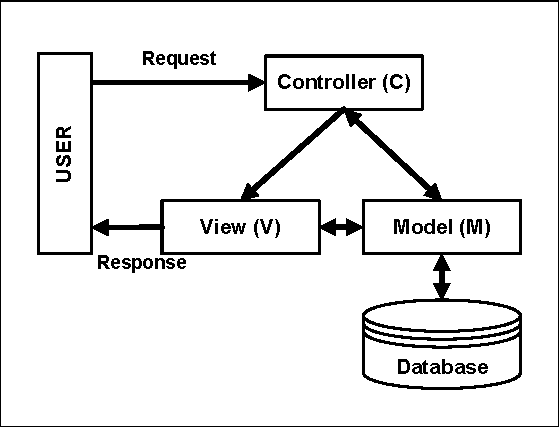
\includegraphics[trim= 10pt 10pt 10pt 10pt, clip, width=8cm]{mvc_fig21.pdf}
		\caption[Mô hình MVC]{\bfseries \fontsize{12pt}{0pt}\selectfont Mô hình MVC}
		\label{fig21}
	\end{figure}
	
	\textbf{Model:} Đây là thành phần chịu trách nhiệm xử lý dữ liệu và logic nghiệp vụ. Model quản lý trạng thái của dữ liệu, tương tác với cơ sở dữ liệu (chẳng hạn như MySQL, SQL Server, SQLite, ...), và thực hiện các thao tác như thêm, sửa, xóa hoặc truy vấn thông tin tài liệu, người dùng, v.v...
	
	\textbf{View:} Thành phần này đại diện cho giao diện người dùng - nơi người dùng tương tác trực tiếp với hệ thống. Trong đề tài, phần View được phát triển bằng ReactJS, hiển thị các dữ liệu như danh sách tài liệu, thông tin chi tiết, giao diện đăng nhập, đăng ký, phân quyền, v.v... View nhận dữ liệu từ Controller và hiển thị lại cho người dùng theo cách trực quan, dễ sử dụng.
	
	\textbf{Controller:} Controller đóng vai trò trung gian giữa Model và View. Nó tiếp nhận các yêu cầu từ người dùng thông qua View (chẳng hạn như thao tác đăng nhập, tìm kiếm tài liệu, tải lên file), xử lý yêu cầu đó bằng cách tương tác với Model, sau đó trả kết quả lại cho View để hiển thị. Trong hệ thống này, Controller được cài đặt ở backend thông qua Node.js và Express, đóng vai trò định tuyến và xử lý logic của ứng dụng.
	
	Việc áp dụng mô hình MVC giúp hệ thống được chia tách rõ ràng theo chức năng, giúp dễ dàng mở rộng, tái sử dụng mã nguồn, và thuận tiện cho việc phát triển theo nhóm hoặc bảo trì lâu dài. Đây là một kiến trúc phù hợp cho các ứng dụng web hiện đại, đặc biệt là các hệ thống có quy mô vừa và lớn.
	
	\subsection{Ngôn ngữ lập trình JavaScript}
	
	JavaScript là một ngôn ngữ lập trình thông dịch, hướng đối tượng, và là một trong ba công nghệ cốt lõi của phát triển web cùng với HTML và CSS. Ban đầu JavaScript được thiết kế để xử lý các tương tác trên trình duyệt phía client (frontend), nhưng với sự phát triển của các công nghệ hiện đại như Node.JS, JavaScript ngày nay còn được sử dụng mạnh mẽ ở phía server (backend), trở thành một ngôn ngữ lập trình toàn diện cho cả hai phía.
	
	Trong đề tài, JavaScript đóng vai trò ngôn ngữ lập trình chính cho cả frontend và backend:
	
	Ở phía frontend, JavaScript được sử dụng kết hợp với thư viện ReactJS để xây dựng giao diện người dùng (UI) tương tác, phản hồi nhanh, và cập nhật linh hoạt theo trạng thái dữ liệu.
	
	Ở phía backend, JavaScript được sử dụng trong môi trường Node.js để xây dựng API, xử lý yêu cầu từ client, truy vấn cơ sở dữ liệu, và quản lý logic nghiệp vụ.
	
	Các ưu điểm chính của JavaScript trong dự án bao gồm:
	\begin{itemize}
		\item Tính nhất quán về ngôn ngữ giữa frontend và backend, giúp đồng bộ logic xử lý và giảm chi phí.
		\item Cộng đồng phát triển mạnh, hỗ trợ thư viện phong phú (npm), dễ mở rộng và tích hợp.
		\item Tốc độ thực thi nhanh, đặc biệt với V8 Engine – giúp backend hoạt động hiệu quả.
		\item Khả năng xử lý bất đồng bộ tốt (với async/await, promise), rất phù hợp với ứng dụng web có nhiều tác vụ I/O như đọc/ghi file, truy vấn database, v.v...
	\end{itemize}
	
	Nhờ sử dụng JavaScript xuyên suốt hệ thống, đề tài có thể phát triển một cách linh hoạt, đồng bộ và dễ bảo trì, đồng thời tận dụng được các công cụ hiện đại hỗ trợ phát triển web hiệu quả hơn.
	
	\subsection{Node.js}
	
	Node.js là một môi trường chạy JavaScript phía máy chủ (server-side), được xây dựng trên nền tảng của Google V8 Engine – trình biên dịch JavaScript hiệu năng cao được sử dụng trong trình duyệt Chrome. Node.js cho phép lập trình viên sử dụng JavaScript để viết các ứng dụng phía backend, từ đó thống nhất ngôn ngữ lập trình giữa frontend và backend.
	
	Một trong những điểm mạnh lớn nhất của Node.js là kiến trúc non-blocking I/O và event-driven (dựa trên sự kiện), giúp xử lý hàng loạt yêu cầu đồng thời một cách hiệu quả mà không làm nghẽn luồng xử lý chính. Điều này đặc biệt phù hợp với các ứng dụng web thời gian thực, ứng dụng cần xử lý nhiều kết nối đồng thời hoặc hệ thống nhẹ mà hiệu năng cao.
	
	Trong khuôn khổ đề tài, Node.js được sử dụng để:
	\begin{itemize}
		\item Xây dựng máy chủ backend phục vụ cho API xử lý logic nghiệp vụ và phản hồi dữ liệu cho frontend.
		\item Tích hợp với framework Express.js nhằm đơn giản hóa việc định tuyến, xử lý yêu cầu và triển khai RESTful API.
		\item Giao tiếp với cơ sở dữ liệu MySQL để lưu trữ và truy xuất thông tin người dùng, tài liệu, và phân quyền.
		\item Xử lý đăng nhập, xác thực, phân quyền truy cập, và quản lý file upload một cách linh hoạt.
	\end{itemize}
	
	Việc sử dụng Node.js giúp hệ thống đạt được hiệu suất cao, giảm độ trễ phản hồi, đồng thời dễ dàng mở rộng và bảo trì nhờ vào cộng đồng phát triển lớn và hệ sinh thái thư viện phong phú (thông qua npm – Node Package Manager).
	
	\subsection{MySQL}
	
	MySQL là một hệ quản trị cơ sở dữ liệu quan hệ (Relational Database Management System – RDBMS) mã nguồn mở, được phát triển và duy trì bởi Oracle Corporation. MySQL sử dụng ngôn ngữ truy vấn SQL (Structured Query Language) để thao tác với dữ liệu, và được sử dụng rộng rãi trong các ứng dụng web nhờ vào khả năng ổn định, hiệu năng tốt và dễ triển khai.
	
	Trong hệ thống quản lý tài liệu học tập của đề tài, MySQL đóng vai trò là cơ sở dữ liệu trung tâm, chịu trách nhiệm lưu trữ và tổ chức toàn bộ dữ liệu của hệ thống.
	
	MySQL hỗ trợ quan hệ giữa các bảng, nhờ đó có thể xây dựng mô hình dữ liệu chặt chẽ và logic, đảm bảo tính toàn vẹn và dễ truy vấn. Trong đề tài, hệ thống sử dụng các thao tác phổ biến như:
	\begin{itemize}
		\item SELECT để truy xuất dữ liệu (tìm kiếm tài liệu, thông tin người dùng).
		\item INSERT, UPDATE, DELETE để thao tác thêm/sửa/xóa dữ liệu.
		\item JOIN để kết nối các bảng liên quan, ví dụ giữa bảng người dùng và bảng tài liệu.
		\item Thiết lập khóa chính – khóa ngoại (Primary Key – Foreign Key) để đảm bảo ràng buộc dữ liệu.
	\end{itemize}
	
	MySQL còn được đánh giá cao vì khả năng tương thích tốt với Node.js thông qua các thư viện như mysql2 hoặc sequelize, cho phép backend giao tiếp với cơ sở dữ liệu một cách nhanh chóng và hiệu quả.
	
	Việc lựa chọn MySQL giúp hệ thống đảm bảo khả năng mở rộng, dễ quản trị và phù hợp với quy mô của ứng dụng web hiện đại hướng đến lưu trữ nhiều tài liệu và người dùng.
	
	\subsection{ReactJS}
	
	ReactJS là một thư viện JavaScript mã nguồn mở được phát triển bởi Facebook, dùng để xây dựng giao diện người dùng (User Interface – UI) cho các ứng dụng web. React hoạt động theo mô hình component-based (thành phần hóa), cho phép chia nhỏ giao diện thành các phần độc lập có thể tái sử dụng, giúp tăng tính linh hoạt, dễ bảo trì và mở rộng hệ thống.
	
	Một trong những điểm nổi bật của React là cơ chế Virtual DOM – giúp tối ưu hiệu suất hiển thị bằng cách chỉ cập nhật các phần tử thay đổi trên giao diện, thay vì render lại toàn bộ trang. Điều này giúp tăng tốc độ phản hồi và cải thiện trải nghiệm người dùng.
	
	Trong đề tài, ReactJS được sử dụng để xây dựng toàn bộ phần giao diện người dùng (frontend), bao gồm các trang như đăng nhập, đăng ký, danh sách tài liệu, form đóng góp tài liệu và phân quyền truy cập. Giao diện này kết nối với backend thông qua các RESTful API được xây dựng bằng Node.js, cho phép gửi và nhận dữ liệu một cách linh hoạt. Bên cạnh đó, React còn hỗ trợ quản lý trạng thái dữ liệu và điều hướng giữa các trang bằng các thư viện tích hợp như React Router, useState, useEffect, giúp giao diện hoạt động mượt mà và phản hồi nhanh chóng.
	
	Các ưu điểm chính khi sử dụng React trong dự án:
	\begin{itemize}
		\item Giao diện hiện đại, tương tác mượt mà và linh hoạt.
		\item Dễ mở rộng và bảo trì nhờ kiến trúc component rõ ràng.
		\item Cộng đồng lớn, hỗ trợ nhiều thư viện và công cụ đi kèm.
		\item Kết hợp tốt với các công nghệ backend như Node.js, Express.
	\end{itemize}
	
	Việc sử dụng React giúp hệ thống không chỉ thân thiện với người dùng mà còn dễ phát triển thêm các tính năng mới, phù hợp với xu hướng phát triển ứng dụng web hiện đại.
	\newpage
	\section*{CHƯƠNG 3. PHÂN TÍCH VÀ THIẾT KẾ HỆ THỐNG}
	\addcontentsline{toc}{section}{\numberline{}CHƯƠNG 3. PHÂN TÍCH VÀ THIẾT KẾ HỆ THỐNG}
	\setcounter{section}{3}
	\setcounter{subsection}{0}
	\setcounter{figure}{0}
	\setcounter{table}{0}
	
	Để xây dựng một hệ thống phần mềm hiệu quả, có tính ứng dụng thực tiễn cao và đáp ứng đúng nhu cầu người dùng, quá trình phân tích và thiết kế hệ thống là bước không thể thiếu. Chương này trình bày các nội dung phân tích và thiết kế cốt lõi nhằm làm rõ phạm vi bài toán, luồng xử lý dữ liệu, chức năng hệ thống cũng như mô hình hóa các thành phần trong hệ thống dưới dạng sơ đồ trực quan.
	
	\subsection{Sơ đồ phân cấp chức năng (FHD)}
	
	Dựa vào các yêu cầu chức năng, ta lập được sơ đồ phân cấp chức năng của hệ thống như Hình \ref{fig31}.
	
	\begin{figure}[!ht]
		\centering
		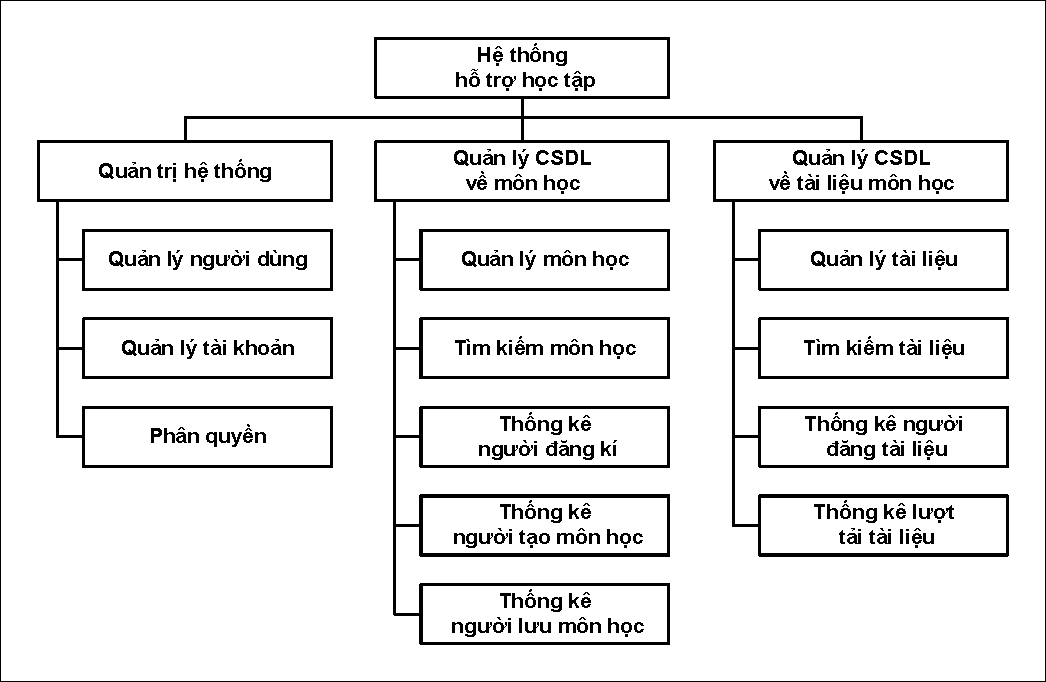
\includegraphics[trim= 10pt 10pt 10pt 10pt, clip, width=16cm]{fhd_fig31_2.pdf}
		\caption [Sơ đồ phân cấp chức năng hệ thống]{\bfseries \fontsize{12pt}{0pt}\selectfont Sơ đồ phân cấp chức năng hệ thống}
		\label{fig31}
	\end{figure}
	
	Hệ thống hỗ trợ học tập được phân chia thành ba phân hệ chính, mỗi phân hệ bao gồm các chức năng cụ thể như sau:
	
	\textbf{Quản trị hệ thống:} Cung cấp các chức năng liên quan đến quản lý người dùng và tài khoản. Người dùng có thể thực hiện đăng ký, chỉnh sửa thông tin cá nhân, thay đổi mật khẩu và được phân quyền truy cập tương ứng theo vai trò (cơ bản, plus, premium). Ngoài ra, hệ thống hỗ trợ giám sát hoạt động của tài khoản và thực hiện các thao tác quản lý hệ thống một cách toàn diện.
	
	\textbf{Quản lý cơ sở dữ liệu về môn học:} Cho phép người dùng quản lý danh sách các môn học, bao gồm thêm mới, chỉnh sửa hoặc xóa thông tin học phần. Hệ thống hỗ trợ tính năng tìm kiếm theo từ khóa và mã môn học nhằm thuận tiện cho việc tra cứu. Ngoài ra, còn có chức năng thống kê số lượng người dùng đã đăng ký học phần và thống kê người dùng đã tạo môn học.
	
	\textbf{Quản lý cơ sở dữ liệu về tài liệu học tập:} Hỗ trợ người dùng quản lý và khai thác hệ thống tài liệu liên quan đến các môn học. Người dùng có thể đăng tải tài liệu mới, chỉnh sửa thông tin tài liệu đã có hoặc tìm kiếm tài liệu theo tên, loại tài liệu hoặc khóa học liên quan. Hệ thống cũng thống kê được số lượng người dùng đã đóng góp tài liệu nhằm đánh giá mức độ tương tác và chia sẻ trong cộng đồng.
	
	\subsection{Sơ đồ luồng dữ liệu (DFD)}
	
	\subsubsection{Mức ngữ cảnh}
	
	Sơ đồ mức ngữ cảnh của hệ thống được mô tả như trên Hình \ref{fig32}. Tiến trình của hệ thống nằm trong mối quan hệ hai thực thể ngoài là: quản trị viên và người dùng. Cụ thể các luồng dữ liệu như sau:
	\begin{figure}[!ht]
		\centering
		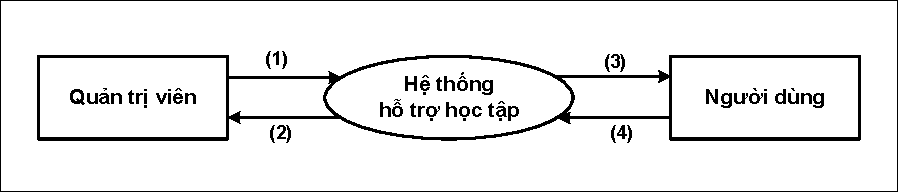
\includegraphics[trim= 10pt 10pt 10pt 10pt, clip, width=15cm]{dfd_fig32.pdf}
		\caption [Sơ đồ luồng dữ liệu mức ngữ cảnh]{\bfseries \fontsize{12pt}{0pt}\selectfont Sơ đồ luồng dữ liệu mức ngữ cảnh}
		\label{fig32}
	\end{figure}
	
	(1) Thông tin các cơ sở dữ liệu liên quan đến người dùng, môn học và tài liệu.

	(2) Tra cứu, quản lý các cơ sở dữ liệu người dùng, môn học và tài liệu.
	
	(3) Thông tin người dùng.
	
	(4) Tra cứu, quản lý người dùng qua các thao tác như thay đổi họ tên, ngày sinh và thay đổi mật khẩu.
	
	\subsubsection{Mức đỉnh}
	
	Sơ đồ luồng dữ liệu mức đỉnh được thể hiện trên Hình \ref{fig33}. Mô hình này có:
	
	\begin{itemize}
		\item Chức năng: Quản trị hệ thống; Quản lý cơ sở dữ liệu về môn học; Quản lý cơ sở dữ liệu về tài liệu học tập.
		\item Tác nhân bên ngoài: Quản trị viên, người dùng.
		\item Kho dữ liệu: a, b.
	\end{itemize}
	
	\begin{figure}[!ht]
		\centering
		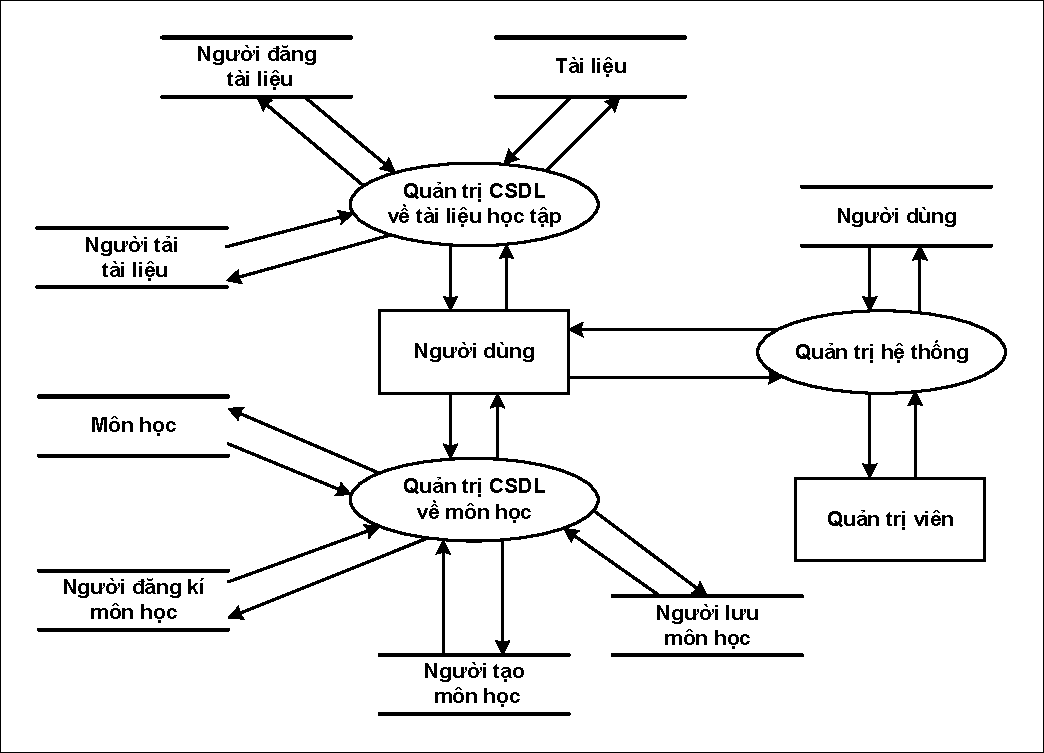
\includegraphics[trim= 10pt 10pt 10pt 10pt, clip, width=15cm]{mucdinh_fig33.pdf}
		\caption [Sơ đồ luồng dữ liệu mức đỉnh]{\bfseries \fontsize{12pt}{0pt}\selectfont Sơ đồ luồng dữ liệu mức đỉnh}
		\label{fig33}
	\end{figure}
	
	\subsubsection{Mức dưới đỉnh}
	\paragraph{Chức năng quản trị hệ thống} \mbox{}
	
	\begin{figure}[!ht]
		\centering
		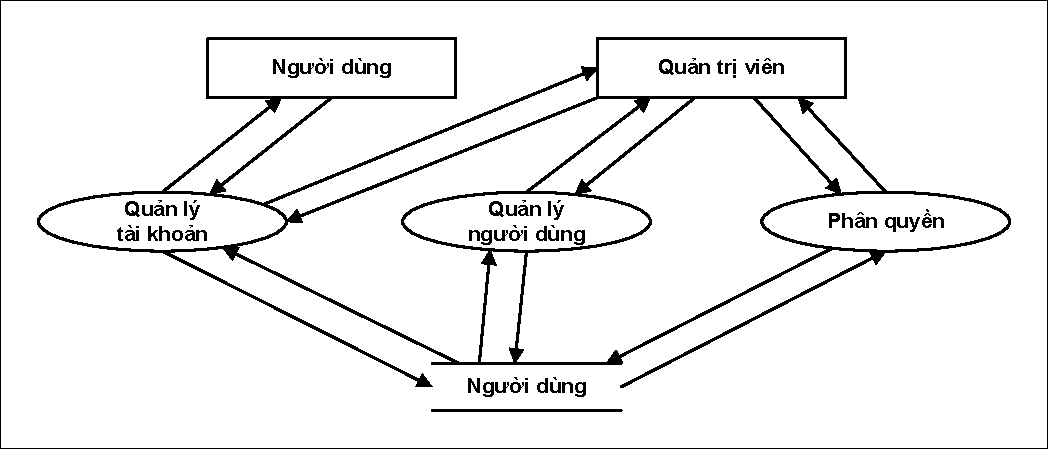
\includegraphics[trim= 10pt 10pt 10pt 10pt, clip, width=15cm]{mucduoidinh_fig34.pdf}
		\caption [Sơ đồ luồng dữ liệu mức dưới đỉnh của chức năng quản trị hệ thống]{\bfseries \fontsize{12pt}{0pt}\selectfont Sơ đồ luồng dữ liệu mức dưới đỉnh của chức năng quản trị hệ thống}
		\label{fig34}
	\end{figure}
	
	Sơ đồ mức dưới đỉnh của chức năng quản trị hệ thống được mô tả trên Hình \ref{fig34}.
	
	\paragraph{Chức năng quản lý CSDL về môn học} \mbox{}
	
	\begin{figure}[!ht]
		\centering
		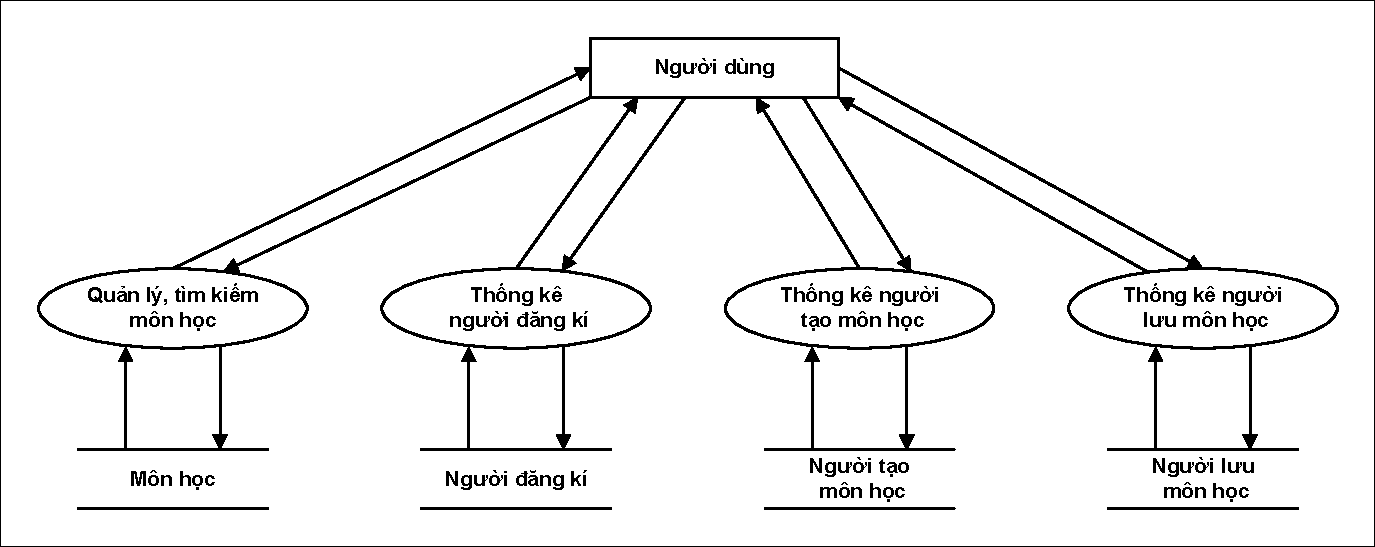
\includegraphics[trim= 10pt 10pt 10pt 10pt, clip, width=16.25cm]{mucduoidinh_fig35.pdf}
		\caption [Sơ đồ luồng dữ liệu mức dưới đỉnh của chức năng quản lý CSDL về môn học]{\bfseries \fontsize{12pt}{0pt}\selectfont Sơ đồ luồng dữ liệu mức dưới đỉnh của chức năng quản lý CSDL về môn học}
		\label{fig35}
	\end{figure}
	
	Sơ đồ mức dưới đỉnh của chức năng quản lý CSDL về môn học được mô tả trên Hình \ref{fig35}.
	
	\paragraph{Chức năng quản lý CSDL về tài liệu môn học} \mbox{}
	
	\begin{figure}[!ht]
		\centering
		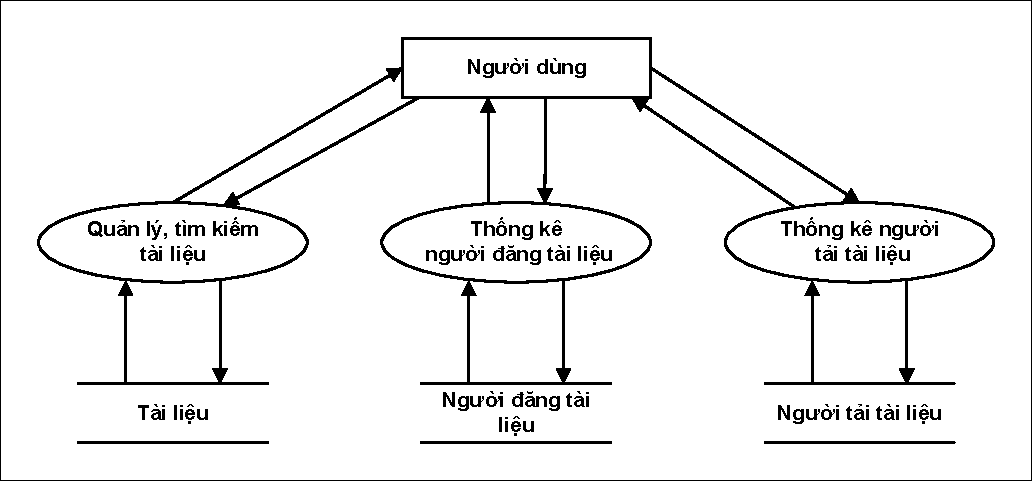
\includegraphics[trim= 10pt 10pt 10pt 10pt, clip, width=16.25cm]{mucduoidinh_fig36.pdf}
		\caption [Sơ đồ luồng dữ liệu mức dưới đỉnh của chức năng quản lý CSDL về tài liệu]{\bfseries \fontsize{12pt}{0pt}\selectfont Sơ đồ luồng dữ liệu mức dưới đỉnh của chức năng quản lý CSDL về tài liệu}
		\label{fig36}
	\end{figure}
	
	Sơ đồ mức dưới đỉnh của chức năng quản lý CSDL về tài liệu học tập được mô tả trên Hình \ref{fig36}.
	
	\subsection{Sơ đồ kịch bản sử dụng (Use Case)}
	
	Hệ thống sẽ bao gồm 3 tác nhân sử dụng hệ thống:
	
	\textbf{Admin:} Là người quản trị toàn hệ thống, có quyền truy cập và thao tác với tất cả các chức năng. Admin có thể quản lý người dùng (xem, tìm kiếm, thêm, chỉnh sửa, xóa tài khoản), phân quyền truy cập, quản lý các môn học, tài liệu và thống kê toàn hệ thống.
	
	\textbf{User:} Có quyền truy cập vào các chức năng cơ bản của hệ thống như xem và tìm kiếm tài liệu, tra cứu thông tin môn học, xem mô tả khóa học, và quản lý thông tin cá nhân của chính mình.
	
	\subsubsection{Danh sách Use Case}
	
		(1) Đăng nhập/Đăng xuất.
		
		(2) Đăng kí (dành cho người dùng mới).
		
		(3) Đăng kí môn học.
		
		(4) Xem thông tin môn học.
		
		(5) Lưu môn học.
		
		(6) Hiển thị và tải tài liệu.
		
		(7) Hiển thị các môn học đã đăng kí.
		
		(8) Hiển thị các môn học đã lưu.
		
		(9) Hiển thị danh sách người dùng (dành cho quản trị viên).
		
		(10) Xóa người dùng (dành cho quản trị viên).
	
	\subsubsection{Sơ đồ Use Case}
	
	\begin{figure}[!ht]
		\centering
		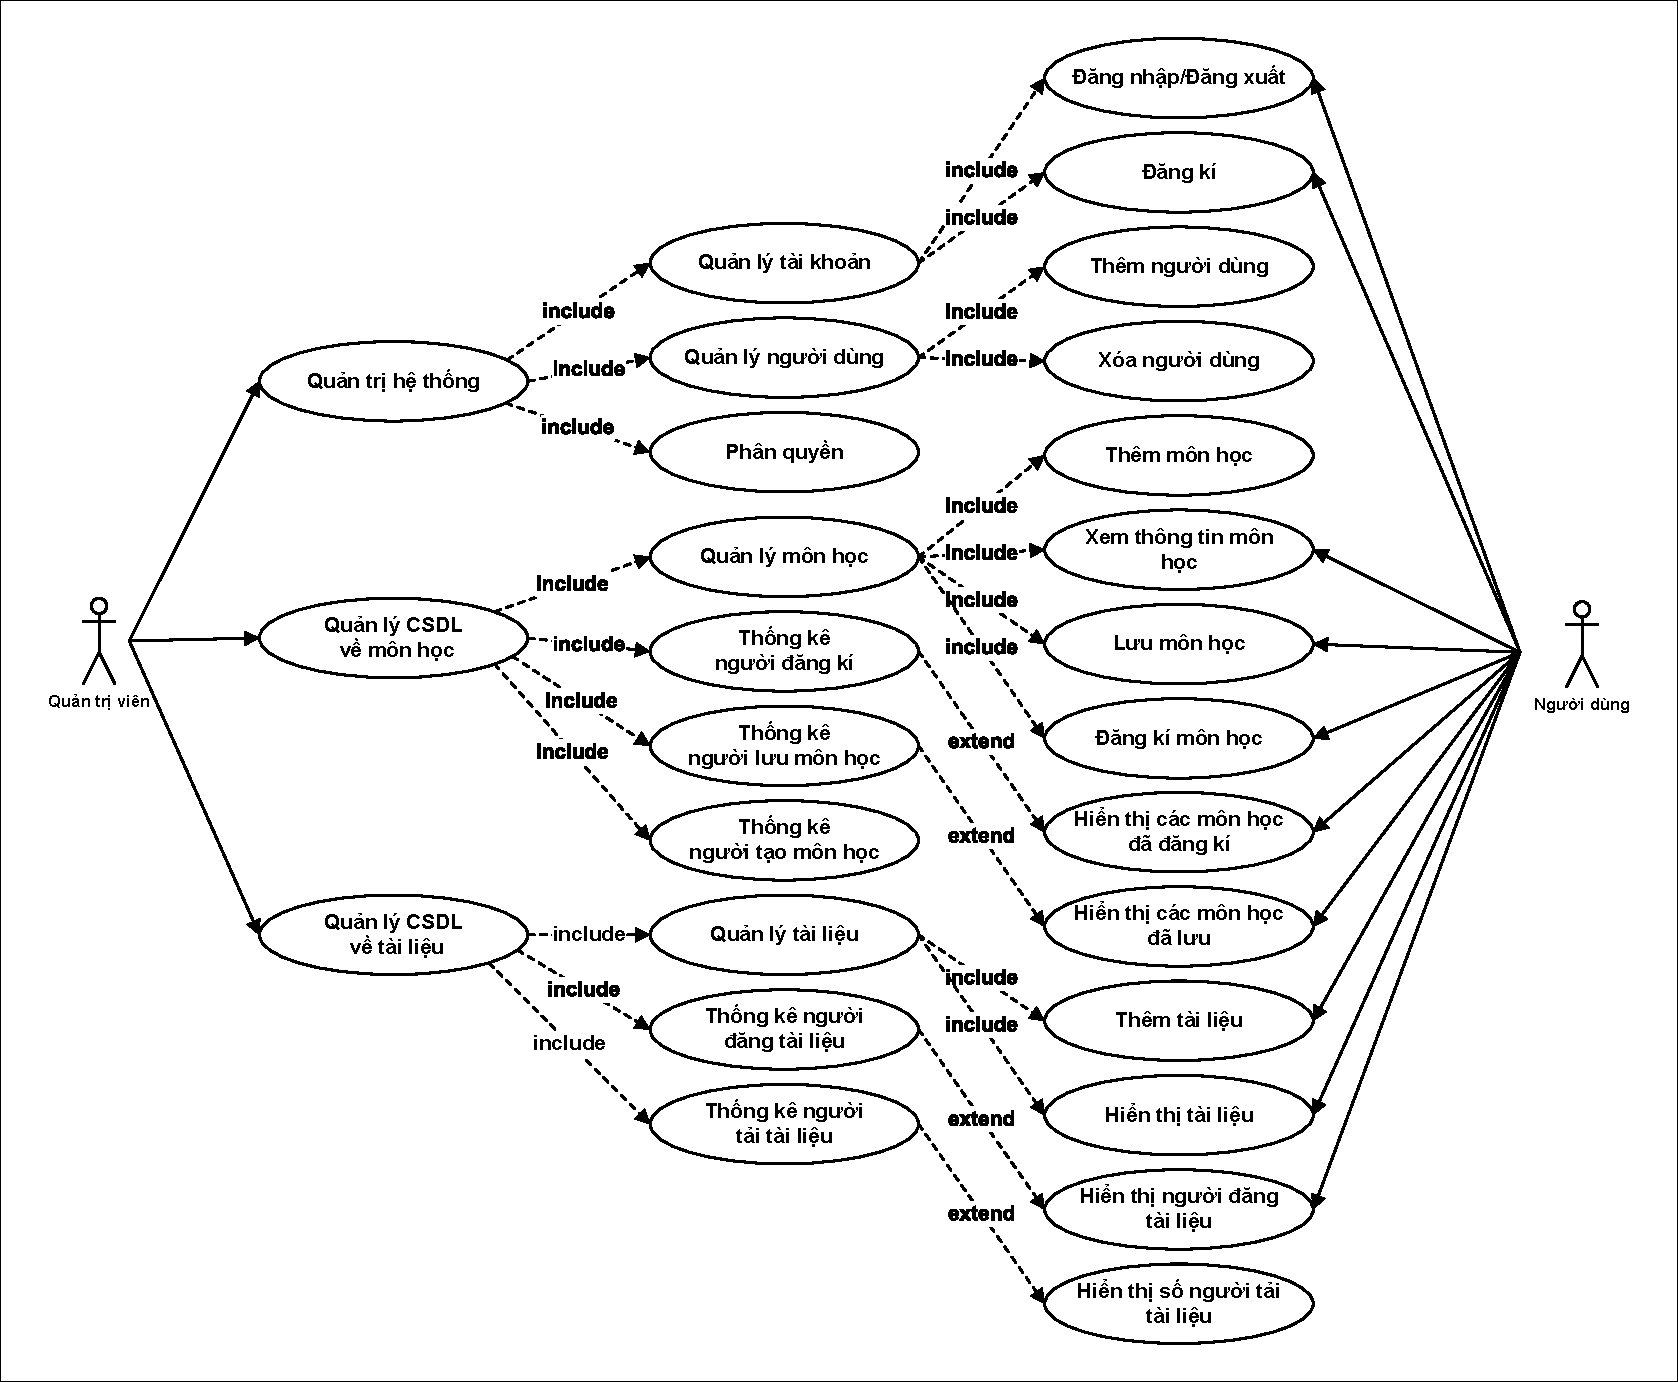
\includegraphics[trim= 10pt 10pt 10pt 10pt, clip, width=16.5cm]{usecase_fig38.pdf}
		\caption [Sơ đồ kịch bản sử dụng (Use Case) chính của hệ thống]{\bfseries \fontsize{12pt}{0pt}\selectfont Sơ đồ kịch bản sử dụng (Use Case) chính của hệ thống}
		\label{fig37}
	\end{figure}
	
	\subsubsection{Đặc tả Use Case}
	
	\paragraph{Đặc tả đăng nhập} \mbox{}
	
	Chức năng Đăng nhập là điểm bắt đầu để người dùng truy cập vào hệ thống hỗ trợ học tập. Đặc tả Use Case của chức năng đăng nhập được thể hiện ở Bảng \ref{tab31}. Thông qua giao diện đăng nhập, người dùng nhập tên đăng nhập (mã số sinh viên) và mật khẩu để xác thực danh tính. Sau khi thông tin được kiểm tra hợp lệ, hệ thống sẽ phân quyền truy cập và chuyển đến giao diện chức năng tương ứng với vai trò của người dùng (quản trị viên, người dùng). Nếu thông tin đăng nhập không chính xác, hệ thống sẽ hiển thị thông báo lỗi và yêu cầu người dùng nhập lại.
	
	\begin{table}[H]
		\centering
		\caption [Đặc tả Use Case Đăng nhập]{\bfseries \fontsize{12pt}{0pt}\selectfont Đặc tả Use Case Đăng nhập}
		\label{tab31}
		\begin{tabular}{|p{4cm}|p{10cm}|}
			\hline
			\textbf{Tên use case} & DangNhap \\
			\hline
			\textbf{Tác nhân chính} & Quản trị viên, Người dùng \\
			\hline
			\textbf{Tiền điều kiện} & Người dùng đã có tài khoản trên hệ thống. \\
			\hline
			\textbf{Đảm bảo tối thiểu} & Hiển thị thông báo lỗi khi đăng nhập thất bại, quay lại giao diện đăng nhập. \\
			\hline
			\textbf{Đảm bảo thành công} & Đăng nhập thành công, chuyển đến giao diện chức năng phù hợp với vai trò. \\
			\hline
			\textbf{Kích hoạt} & Người dùng nhấn nút “Đăng nhập” trên giao diện hệ thống. \\
			\hline
			\textbf{Chuỗi sự kiện chính} &
			- Người dùng nhập username và password.
			
			- Nhấn nút “Đăng nhập”.
			
			- Hệ thống kiểm tra thông tin đăng nhập.
			
			- Nếu hợp lệ, chuyển hướng tới giao diện tương ứng theo phân quyền.
			\\
			\hline
			\textbf{Ngoại lệ} &
			- Tài khoản không tồn tại.
			
			- Mật khẩu không đúng.
			
			- Hệ thống báo lỗi và giữ lại giao diện đăng nhập.
			\\
			\hline
		\end{tabular}
	\end{table}

	\paragraph{Đặc tả đăng ký} \mbox{}
	
	Đặc tả Use Case của chức năng đăng ký được thể hiện ở Bảng \ref{tab32}. Thông qua biểu mẫu đăng ký, người dùng nhập các thông tin cá nhân cơ bản như họ tên, mã số sinh viên và mật khẩu. Hệ thống sẽ kiểm tra tính hợp lệ và đảm bảo rằng các thông tin như email hoặc tên đăng nhập chưa bị trùng lặp. Sau khi đăng ký thành công, người dùng sẽ được chuyển đến giao diện đăng nhập để bắt đầu sử dụng hệ thống.
	
	\begin{table}[H]
		\centering
		\caption [Đặc tả Use Case Đăng ký]{\bfseries \fontsize{12pt}{0pt}\selectfont Đặc tả Use Case Đăng ký}
		\label{tab32}
		\begin{tabular}{|p{4cm}|p{10.5cm}|}
			\hline
			\textbf{Tên use case} & DangKy \\
			\hline
			\textbf{Tác nhân chính} & Người dùng \\
			\hline
			\textbf{Tiền điều kiện} & Người dùng chưa có tài khoản trên hệ thống. \\
			\hline
			\textbf{Đảm bảo tối thiểu} & Hệ thống thông báo lỗi nếu thiếu hoặc sai định dạng thông tin. \\
			\hline
			\textbf{Đảm bảo thành công} & Tạo tài khoản thành công, chuyển hướng đến giao diện đăng nhập. \\
			\hline
			\textbf{Kích hoạt} & Người dùng truy cập trang đăng ký và nhấn nút “Đăng ký”. \\
			\hline
			\textbf{Chuỗi sự kiện chính} &
			- Người dùng truy cập giao diện đăng ký.
			
			- Nhập đầy đủ thông tin: họ tên, email, tên đăng nhập, mật khẩu.
			
			- Nhấn nút "Đăng ký".
			
			- Hệ thống kiểm tra hợp lệ và tạo tài khoản mới.
			
			- Chuyển đến giao diện đăng nhập.
			\\
			\hline
			\textbf{Ngoại lệ} &
			- Thiếu thông tin bắt buộc (họ tên, mã số sinh viên, mật khẩu).
			
			- Email hoặc tên đăng nhập đã tồn tại.
			
			- Hệ thống hiển thị thông báo lỗi và giữ lại thông tin đã nhập.
			\\
			\hline
		\end{tabular}
	\end{table}
	
	\paragraph{Đặc tả đăng ký môn học} \mbox{}
	
	Đặc tả Use Case của chức năng đăng ký môn học được thể hiện ở Bảng \ref{tab33}. Người dùng có thể tìm học phần tỏng danh sách học phần, sau đó thực hiện đăng ký chỉ với một thao tác. Hệ thống sẽ kiểm tra tính hợp lệ (tránh đăng ký trùng lặp) trước khi lưu vào cơ sở dữ liệu cá nhân của người dùng.
	
	\begin{table}[H]
		\centering
		\caption [Đặc tả Use Case Đăng ký môn học]{\bfseries \fontsize{12pt}{0pt}\selectfont Đặc tả Use Case Đăng ký môn học}
		\label{tab33}
		\begin{tabular}{|p{4cm}|p{10.5cm}|}
			\hline
			\textbf{Tên use case} & DangKyMonHoc \\
			\hline
			\textbf{Tác nhân chính} & Người dùng \\
			\hline
			\textbf{Tiền điều kiện} & Người dùng đã đăng nhập thành công vào hệ thống. \\
			\hline
			\textbf{Đảm bảo tối thiểu} & Hiển thị đăng ký thành công \\
			\hline
			\textbf{Đảm bảo thành công} & Môn học được lưu vào danh sách đăng ký cá nhân của người dùng. \\
			\hline
			\textbf{Kích hoạt} & Người dùng truy cập giao diện đăng ký môn học. \\
			\hline
			\textbf{Chuỗi sự kiện chính} &
			- Người dùng vào trang danh sách học phần.
			
			- Chọn môn học cần đăng ký.
			
			- Nhấn nút "Đăng ký học phần".
			
			- Hệ thống kiểm tra môn học đã được đăng ký hay chưa.
			
			- Nếu chưa, lưu thông tin vào cơ sở dữ liệu người dùng.
			\\
			\hline
			\textbf{Ngoại lệ} &
			- Người dùng chưa chọn môn nào.
			
			- Môn học đã được đăng ký từ trước.
			\\
			\hline
		\end{tabular}
	\end{table}
	
	\paragraph{Đặc tả xem thông tin môn học} \mbox{}
	
	\begin{table}[H]
		\centering
		\caption [Đặc tả Use Case Xem thông tin môn học]{\bfseries \fontsize{12pt}{0pt}\selectfont Đặc tả Use Case Xem thông tin môn học}
		\label{tab34}
		\begin{tabular}{|p{4cm}|p{10.5cm}|}
			\hline
			\textbf{Tên use case} & XemThongTinMonHoc \\
			\hline
			\textbf{Tác nhân chính} & Người dùng \\
			\hline
			\textbf{Tiền điều kiện} & Người dùng đã đăng nhập vào hệ thống. \\
			\hline
			\textbf{Đảm bảo tối thiểu} & Nếu mã môn học không tồn tại, hệ thống hiển thị thông báo lỗi. \\
			\hline
			\textbf{Đảm bảo thành công} & Thông tin chi tiết của môn học được hiển thị chính xác và đầy đủ. \\
			\hline
			\textbf{Kích hoạt} & Người dùng nhấn chọn một môn học bất kỳ từ danh sách môn học. \\
			\hline
			\textbf{Chuỗi sự kiện chính} &
			- Người dùng truy cập danh sách các môn học.
			
			- Chọn một môn cụ thể muốn xem chi tiết.
			
			- Hệ thống lấy thông tin môn học từ cơ sở dữ liệu.
			
			- Hiển thị thông tin chi tiết như tên môn, mã, mô tả, số tín chỉ, đơn vị quản lý,...
			\\
			\hline
			\textbf{Ngoại lệ} &
			- Mã môn học không tồn tại trong cơ sở dữ liệu.
			
			- Có lỗi khi truy xuất thông tin từ backend hoặc API không phản hồi.
			\\
			\hline
		\end{tabular}
	\end{table}
	
	Đặc tả Use Case của chức năng xem thông tin môn học được thể hiện ở Bảng \ref{tab34}. Chức năng Xem thông tin môn học cho phép người dùng truy cập chi tiết vào nội dung của một học phần cụ thể. Tính năng này giúp người học nắm được các thông tin quan trọng như tên môn, mã môn, mô tả, số tín chỉ, v.v ... 
	
	\paragraph{Đặc tả lưu môn học} \mbox{}
	
	Đặc tả Use Case của chức năng lưu môn học được thể hiện ở Bảng \ref{tab35}. Chức năng Lưu môn học cho phép người dùng đánh dấu những môn học mà họ quan tâm đặc biệt hơn. Mục đích của chức năng này là giúp người dùng thuận tiện hơn trong việc quay lại xem môn học, đồng thời tạo ra danh sách các học phần được theo dõi riêng.
	
	\begin{table}[H]
		\centering
		\caption [Đặc tả Use Case Lưu môn học]{\bfseries \fontsize{12pt}{0pt}\selectfont Đặc tả Use Case Lưu môn học}
		\label{tab35}
		\begin{tabular}{|p{4cm}|p{10.5cm}|}
			\hline
			\textbf{Tên use case} & LuuMonHoc \\
			\hline
			\textbf{Tác nhân chính} & Người dùng \\
			\hline
			\textbf{Tiền điều kiện} & Người dùng đã đăng nhập và đang xem thông tin chi tiết một môn học. \\
			\hline
			\textbf{Đảm bảo tối thiểu} & Hệ thống hiển thị thông báo nếu môn học đã được lưu trước đó. \\
			\hline
			\textbf{Đảm bảo thành công} & Môn học được thêm vào danh sách môn học đã lưu của người dùng. \\
			\hline
			\textbf{Kích hoạt} & Người dùng nhấn nút “Lưu môn học” tại trang thông tin chi tiết môn học. \\
			\hline
			\textbf{Chuỗi sự kiện chính} &
			- Người dùng truy cập danh sách môn học.
			
			- Nhấn nút “Lưu môn học”.
			
			- Hệ thống kiểm tra xem môn đã được lưu chưa.
			
			- Nếu chưa, lưu mã môn vào danh sách cá nhân trong cơ sở dữ liệu.
			
			- Hiển thị thông báo lưu thành công.
			\\
			\hline
			\textbf{Ngoại lệ} &
			- Môn học đã tồn tại trong danh sách lưu.
			
			- Lỗi kết nối cơ sở dữ liệu hoặc backend không phản hồi.
			\\
			\hline
		\end{tabular}
	\end{table}
	
	\paragraph{Đặc tả hiển thị và tải tài liệu} \mbox{}
	
	Đặc tả Use Case của chức năng hiển thị và tải tài liệu được thể hiện ở Bảng \ref{tab36}. Chức năng Hiển thị và Tải tài liệu cho phép người dùng truy cập danh sách tài liệu liên quan đến các môn học mà họ đã đăng ký hoặc lưu trước đó. Hệ thống cung cấp tên tài liệu, mô tả ngắn, người đóng góp và liên kết tải xuống. Người dùng có thể dễ dàng duyệt qua các tài liệu sẵn có và lựa chọn những tài liệu phù hợp để tải về máy.
	
	\begin{table}[H]
		\centering
		\caption [Đặc tả Use Case Hiển thị và tải tài liệu]{\bfseries \fontsize{12pt}{0pt}\selectfont Đặc tả Use Case Hiển thị và tải tài liệu}
		\label{tab36}
		\begin{tabular}{|p{4cm}|p{10.5cm}|}
			\hline
			\textbf{Tên use case} & HienThiVaTaiTaiLieu \\
			\hline
			\textbf{Tác nhân chính} & Người dùng \\
			\hline
			\textbf{Tiền điều kiện} & Người dùng đã đăng nhập và có quyền truy cập vào tài liệu theo cấp độ tài khoản. \\
			\hline
			\textbf{Đảm bảo tối thiểu} & Hệ thống vẫn hiển thị nếu không có tài liệu nào (hiển thị thông báo "Không có tài liệu phù hợp"). \\
			\hline
			\textbf{Đảm bảo thành công} & Danh sách tài liệu hiển thị chính xác, người dùng có thể tải xuống file tương ứng. \\
			\hline
			\textbf{Kích hoạt} & Người dùng truy cập trang tài liệu hoặc mục tài liệu trong thông tin môn học. \\
			\hline
			\textbf{Chuỗi sự kiện chính} &
			- Người dùng truy cập vào danh sách môn học, hoặc tìm kiếm theo tên.
			
			- Hệ thống truy vấn các tài liệu theo môn học.
			
			- Hiển thị thông tin tài liệu: tên, người đăng, ngày đăng,...
			
			- Người dùng chọn tài liệu để tải.
			
			- Hệ thống cung cấp liên kết tải file về máy.
			\\
			\hline
			\textbf{Ngoại lệ} &
			- Không có tài liệu phù hợp với môn học.
			
			- Lỗi kết nối cơ sở dữ liệu hoặc file bị lỗi không thể tải.
			\\
			\hline
		\end{tabular}
	\end{table}
	
	\paragraph{Đặc tả hiển thị các môn học đã đăng kí} \mbox{}
	
	Đặc tả Use Case của chức năng hiển thị các môn học đã đăng kí được thể hiện ở Bảng \ref{tab37}. Chức năng Hiển thị các môn học đã đăng ký giúp người dùng dễ dàng theo dõi danh sách các học phần mà họ đã chọn trước đó. Tính năng này hỗ trợ việc truy cập nhanh vào các môn học đang quan tâm, từ đó người dùng có thể xem tài liệu, cập nhật thông tin hoặc hủy đăng ký nếu cần. Danh sách được cá nhân hóa theo tài khoản và được hệ thống lưu trữ liên tục trong quá trình sử dụng.
	
	\begin{table}[H]
		\centering
		\caption [Đặc tả Use Case Hiển thị các môn học đã đăng kí]{\bfseries \fontsize{12pt}{0pt}\selectfont Đặc tả Use Case Hiển thị các môn học đã đăng kí}
		\label{tab37}
		\begin{tabular}{|p{4cm}|p{10.5cm}|}
			\hline
			\textbf{Tên use case} & HienThiMonHocDaDangKy \\
			\hline
			\textbf{Tác nhân chính} & Người dùng \\
			\hline
			\textbf{Tiền điều kiện} & Người dùng đã đăng nhập và có ít nhất một môn học đã đăng ký. \\
			\hline
			\textbf{Đảm bảo tối thiểu} & Nếu chưa đăng ký môn học nào, hệ thống hiển thị thông báo tương ứng. \\
			\hline
			\textbf{Đảm bảo thành công} & Hiển thị đúng danh sách môn học đã đăng ký theo tài khoản người dùng. \\
			\hline
			\textbf{Kích hoạt} & Người dùng truy cập mục “Môn học đã đăng ký” trên giao diện hệ thống. \\
			\hline
			\textbf{Chuỗi sự kiện chính} &
			- Người dùng truy cập mục “Môn học đã đăng ký”.
			
			- Hệ thống truy vấn các môn học từ cơ sở dữ liệu dựa theo ID người dùng.
			
			- Hiển thị danh sách các môn đã đăng ký: tên môn, mã môn, ...
			\\
			\hline
			\textbf{Ngoại lệ} &
			- Người dùng chưa đăng ký môn học nào.
			
			- Lỗi truy xuất dữ liệu từ cơ sở dữ liệu hoặc API.
			\\
			\hline
		\end{tabular}
	\end{table}
	
	\paragraph{Đặc tả hiển thị các môn học đã lưu} \mbox{}
	
	Đặc tả Use Case của chức năng hiển thị các môn học đã lưu được thể hiện ở Bảng \ref{tab38}. Chức năng Hiển thị các môn học đã lưu giúp người dùng dễ dàng theo dõi các học phần mà họ đã đánh dấu quan tâm. Tính năng này hỗ trợ người học trong việc ghi nhớ các môn quan trọng, đồng thời cho phép truy cập nhanh đến thông tin chi tiết. Danh sách được lưu trữ cá nhân hóa cho từng tài khoản và có thể cập nhật liên tục trong quá trình sử dụng.
	
	\begin{table}[H]
		\centering
		\caption [Đặc tả Use Case Hiển thị các môn học đã lưu]{\bfseries \fontsize{12pt}{0pt}\selectfont Đặc tả Use Case Hiển thị các môn học đã lưu}
		\label{tab38}
		\begin{tabular}{|p{4cm}|p{10.5cm}|}
			\hline
			\textbf{Tên use case} & HienThiMonHocDaDangKy \\
			\hline
			\textbf{Tác nhân chính} & Người dùng \\
			\hline
			\textbf{Tiền điều kiện} & Người dùng đã đăng nhập và có ít nhất một môn học đã lưu. \\
			\hline
			\textbf{Đảm bảo tối thiểu} & Nếu chưa lưu môn học nào, hệ thống hiển thị thông báo tương ứng. \\
			\hline
			\textbf{Đảm bảo thành công} & Hiển thị đúng danh sách môn học đã lưu theo tài khoản người dùng. \\
			\hline
			\textbf{Kích hoạt} & Người dùng truy cập mục “Môn học đã lưu” trên giao diện hệ thống. \\
			\hline
			\textbf{Chuỗi sự kiện chính} &
			- Người dùng truy cập mục “Môn học đã lưu”.
			
			- Hệ thống truy vấn các môn học từ cơ sở dữ liệu dựa theo ID người dùng.
			
			- Hiển thị danh sách các môn đã lưu: tên môn, mã môn, ...
			\\
			\hline
			\textbf{Ngoại lệ} &
			- Người dùng chưa lưu môn học nào.
			
			- Lỗi truy xuất dữ liệu từ cơ sở dữ liệu hoặc API.
			\\
			\hline
		\end{tabular}
	\end{table}
	
	\paragraph{Đặc tả hiển thị danh sách người dùng (dành cho quản trị viên)} \mbox{}
	
	\begin{table}[H]
		\centering
		\caption [Đặc tả Use Case Hiển thị danh sách người dùng]{\bfseries \fontsize{12pt}{0pt}\selectfont Đặc tả Use Case Hiển thị danh sách người dùng}
		\label{tab39}
		\begin{tabular}{|p{4cm}|p{10.5cm}|}
			\hline
			\textbf{Tên use case} & HienThiDanhSachNguoiDung \\
			\hline
			\textbf{Tác nhân chính} & Quản trị viên (Admin) \\
			\hline
			\textbf{Tiền điều kiện} & Quản trị viên đã đăng nhập vào hệ thống bằng tài khoản hợp lệ. \\
			\hline
			\textbf{Đảm bảo tối thiểu} & Nếu không có người dùng nào, hệ thống hiển thị danh sách trống với thông báo phù hợp. \\
			\hline
			\textbf{Đảm bảo thành công} & Hiển thị đầy đủ danh sách người dùng, bao gồm thông tin cơ bản và phân quyền. \\
			\hline
			\textbf{Kích hoạt} & Quản trị viên chọn mục “Quản lý người dùng”. \\
			\hline
			\textbf{Chuỗi sự kiện chính} &
			- Quản trị viên chọn mục “Quản lý người dùng”.
			
			- Hệ thống truy vấn danh sách người dùng từ cơ sở dữ liệu.
			
			- Hiển thị danh sách bao gồm: username, họ tên, giới tính, ngày sinh, quyền truy cập, trạng thái tài khoản.
			\\
			\hline
			\textbf{Ngoại lệ} &
			- Lỗi truy vấn cơ sở dữ liệu.
			
			- Danh sách không hiển thị do lỗi phân quyền hoặc mất phiên đăng nhập.
			\\
			\hline
		\end{tabular}
	\end{table}
	
	Đặc tả Use Case của chức năng hiển thị danh sách người dùng được thể hiện ở Bảng \ref{tab39}. Chức năng Hiển thị danh sách người dùng cho phép quản trị viên truy cập toàn bộ thông tin người dùng đang sử dụng hệ thống. Tính năng này hỗ trợ việc giám sát, theo dõi hoạt động người dùng, kiểm tra phân quyền truy cập và thực hiện các thao tác quản lý như chỉnh sửa hoặc vô hiệu hóa tài khoản. Giao diện được thiết kế đơn giản, rõ ràng, cung cấp các thông tin cơ bản như tên đăng nhập, họ tên, email, loại tài khoản, ngày đăng ký,… để quản trị viên thao tác hiệu quả.
	
	\paragraph{Đặc tả xóa người dùng (dành cho quản trị viên)} \mbox{}
	
	Đặc tả Use Case của chức năng xóa người dùng được thể hiện ở Bảng \ref{tab310}. Chức năng Xóa người dùng cho phép quản trị viên loại bỏ một tài khoản khỏi hệ thống trong trường hợp tài khoản đó vi phạm quy định, không còn sử dụng hoặc theo yêu cầu quản lý. Trước khi xóa, hệ thống có thể hiển thị hộp thoại xác nhận nhằm đảm bảo tính chính xác và tránh thao tác nhầm. Việc xóa tài khoản sẽ đồng thời loại bỏ quyền truy cập của người dùng và đảm bảo dữ liệu liên quan được xử lý phù hợp theo chính sách hệ thống.
	
	\begin{table}[H]
		\centering
		\caption [Đặc tả Use Case Xóa người dùng]{\bfseries \fontsize{12pt}{0pt}\selectfont Đặc tả Use Case Xóa người dùng}
		\label{tab310}
		\begin{tabular}{|p{4cm}|p{10.5cm}|}
			\hline
			\textbf{Tên use case} & XoaNguoiDung \\
			\hline
			\textbf{Tác nhân chính} & Quản trị viên (Admin) \\
			\hline
			\textbf{Tiền điều kiện} & Quản trị viên đã đăng nhập và đang ở trong giao diện quản lý người dùng. \\
			\hline
			\textbf{Đảm bảo tối thiểu} & Nếu không chọn người dùng, hệ thống không thực hiện thao tác xóa và hiển thị cảnh báo. \\
			\hline
			\textbf{Đảm bảo thành công} & Tài khoản người dùng được xóa khỏi hệ thống, và không còn quyền truy cập. \\
			\hline
			\textbf{Kích hoạt} & Quản trị viên chọn người dùng cụ thể và nhấn nút “Xóa tài khoản”. \\
			\hline
			\textbf{Chuỗi sự kiện chính} &
			- Quản trị viên truy cập danh sách người dùng.
			
			- Chọn một người dùng cụ thể muốn xóa.
			
			- Nhấn “Xóa” và xác nhận thao tác.
			
			- Hệ thống kiểm tra và thực hiện xóa tài khoản khỏi cơ sở dữ liệu.
			
			- Hiển thị thông báo “Xóa thành công”.
			\\
			\hline
			\textbf{Ngoại lệ} &
			- Không chọn người dùng hoặc thao tác bị hủy.
			
			- Lỗi kết nối đến cơ sở dữ liệu hoặc không đủ quyền xóa.
			\\
			\hline
		\end{tabular}
	\end{table}
	
	\subsection{Biểu đồ Activity Diagram}
	\subsubsection{Chức năng đăng nhập}
	
	Biểu đồ hoạt động luồng xử lý chức năng đăng nhập trong hệ thống được biểu diễn trên Hình \ref{fig39}. Khi người dùng truy cập và nhập thông tin đăng nhập (gồm tên đăng nhập và mật khẩu), hệ thống sẽ tiến hành kiểm tra tính hợp lệ của các thông tin này. Nếu tài khoản tồn tại và thông tin là chính xác, hệ thống sẽ chuyển người dùng đến trang chủ hoặc giao diện chức năng phù hợp với vai trò (ví dụ: người dùng thường hoặc quản trị viên). Ngược lại, nếu thông tin đăng nhập không hợp lệ, hệ thống sẽ thông báo lỗi và yêu cầu người dùng đăng nhập lại. Quy trình này giúp đảm bảo tính bảo mật, chỉ cho phép truy cập đối với những tài khoản hợp lệ.
	
	\begin{figure}[!ht]
		\centering
		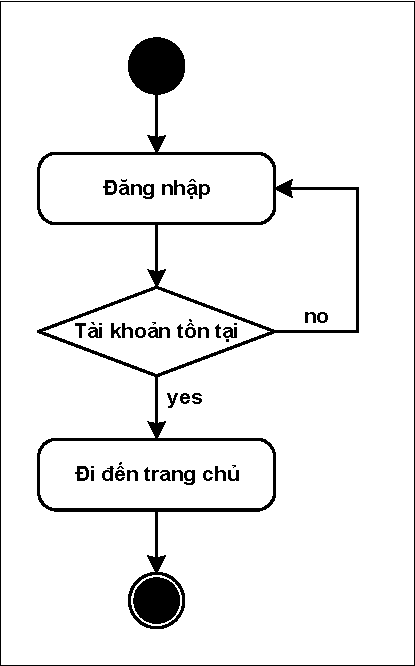
\includegraphics[trim= 10pt 10pt 10pt 10pt, clip, width=6.5cm]{activity_fig39.pdf}
		\caption [Biểu đồ Activity Diagram luồng đăng nhập]{\bfseries \fontsize{12pt}{0pt}\selectfont Biểu đồ Activity Diagram luồng đăng nhập}
		\label{fig39}
	\end{figure}
	
	\subsubsection{Chức năng đăng ký}
	
	Biểu đồ hoạt động luồng xử lý chức năng đăng ký trong hệ thống được biểu diễn trên Hình \ref{fig310}. Quá trình bắt đầu khi người dùng truy cập trang đăng ký và tiến hành điền đầy đủ các thông tin yêu cầu trong biểu mẫu (form). Sau đó, hệ thống thực hiện bước kiểm tra tính hợp lệ của thông tin đầu vào như: độ dài mật khẩu, xác thực lại mật khẩu, kiểm tra trùng tên người dùng, v.v. Nếu thông tin không hợp lệ, người dùng được yêu cầu nhập lại. Trường hợp tất cả thông tin đều hợp lệ, tài khoản sẽ được tạo thành công và người dùng được chuyển hướng đến trang đăng nhập để tiếp tục sử dụng hệ thống. 
	
	\begin{figure}[!ht]
		\centering
		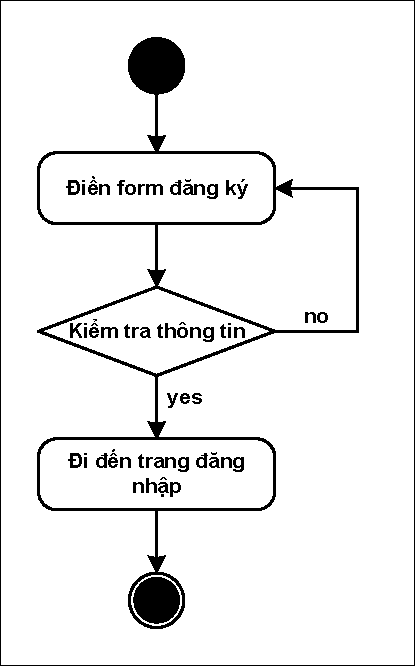
\includegraphics[trim= 10pt 10pt 10pt 10pt, clip, width=6.5cm]{activity_fig310.pdf}
		\caption [Biểu đồ Activity Diagram luồng đăng ký]{\bfseries \fontsize{12pt}{0pt}\selectfont Biểu đồ Activity Diagram luồng đăng ký}
		\label{fig310}
	\end{figure}
	
	\subsubsection{Chức năng đăng ký môn học}
	
	Biểu đồ hoạt động luồng xử lý chức năng đăng ký môn học trong hệ thống được biểu diễn trên Hình \ref{fig311}. Quá trình bắt đầu khi người dùng lựa chọn thao tác “Đăng ký môn học”. Hệ thống sẽ kiểm tra trạng thái đăng nhập: nếu người dùng chưa đăng nhập, hệ thống sẽ điều hướng họ về trang đăng nhập để xác thực. Sau khi đăng nhập thành công, hệ thống tiến hành tra cứu danh sách các môn học mà người dùng đã đăng ký. Nếu môn học đã tồn tại trong danh sách đăng ký, quá trình sẽ kết thúc và không thực hiện thao tác lặp lại. Ngược lại, nếu môn học chưa được đăng ký, hệ thống sẽ thêm môn học đó vào danh sách đã đăng ký của người dùng.
		
	\begin{figure}[!ht]
		\centering
		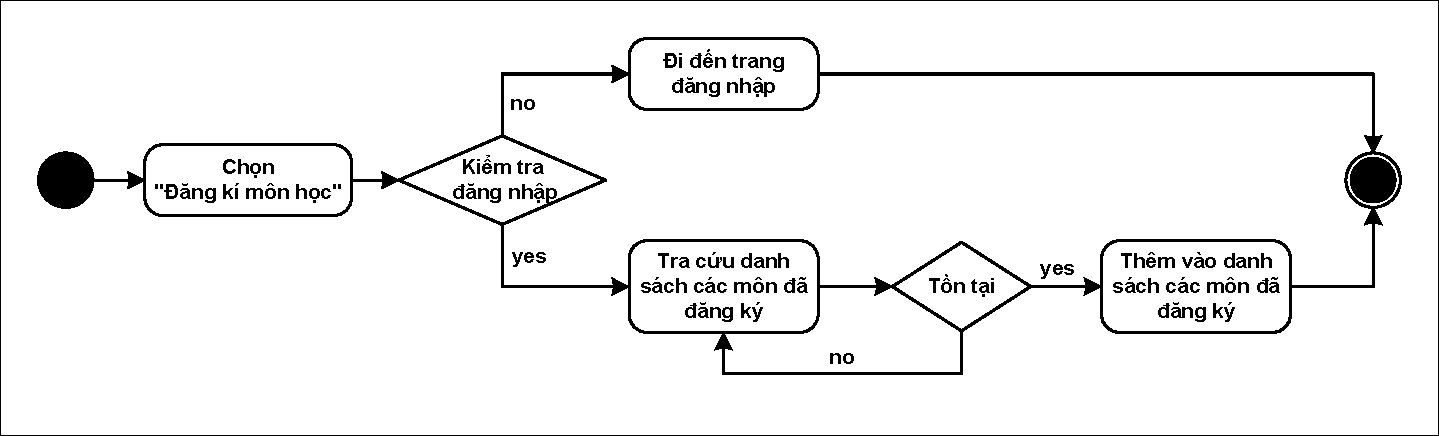
\includegraphics[trim= 10pt 10pt 10pt 10pt, clip, width=16cm]{activity_fig311.pdf}
		\caption [Biểu đồ Activity Diagram luồng đăng ký môn học]{\bfseries \fontsize{12pt}{0pt}\selectfont Biểu đồ Activity Diagram luồng đăng ký môn học}
		\label{fig311}
	\end{figure}
	
	\subsubsection{Chức năng lưu môn học}
	
	Biểu đồ hoạt động luồng xử lý chức năng lưu môn học trong hệ thống được biểu diễn trên Hình \ref{fig312}. Quá trình bắt đầu khi người dùng lựa chọn thao tác “Lưu môn học”. Hệ thống sẽ kiểm tra trạng thái đăng nhập: nếu người dùng chưa đăng nhập, hệ thống sẽ điều hướng họ về trang đăng nhập để xác thực. Sau khi đăng nhập thành công, hệ thống tiến hành tra cứu danh sách các môn học mà người dùng đã lưu. Nếu môn học đã tồn tại trong danh sách đã lưu, quá trình sẽ kết thúc và không thực hiện thao tác lặp lại. Ngược lại, nếu môn học chưa được lưu, hệ thống sẽ thêm môn học đó vào danh sách đã lưu của người dùng.
	
	\begin{figure}[!ht]
		\centering
		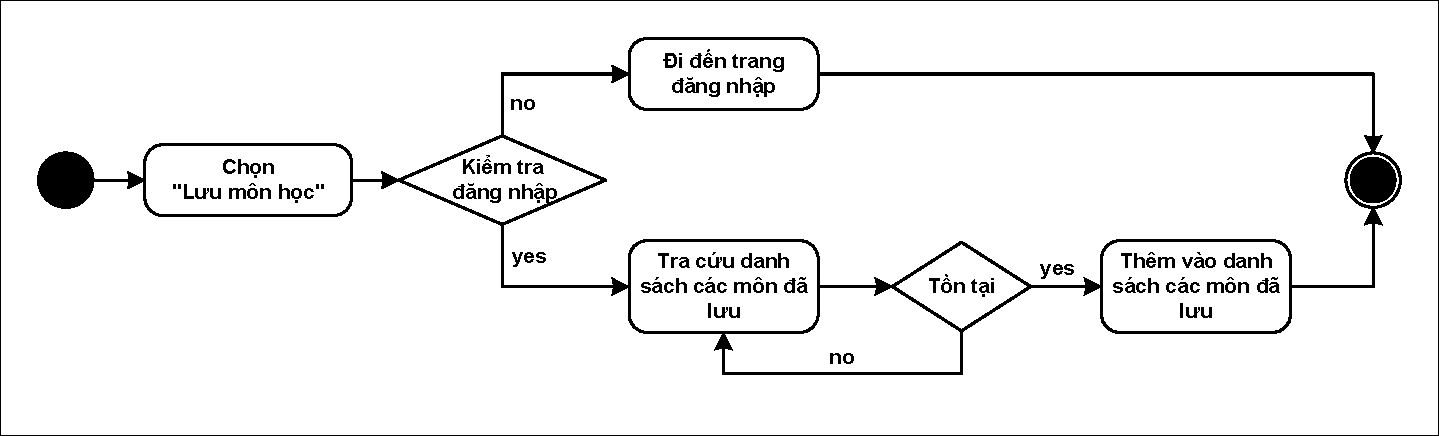
\includegraphics[trim= 10pt 10pt 10pt 10pt, clip, width=16cm]{activity_fig312.pdf}
		\caption [Biểu đồ Activity Diagram luồng lưu môn học]{\bfseries \fontsize{12pt}{0pt}\selectfont Biểu đồ Activity Diagram luồng lưu môn học}
		\label{fig312}
	\end{figure}
	
	\subsubsection{Chức năng hiển thị danh sách người dùng}
	
	Biểu đồ hoạt động luồng xử lý chức năng hiển thị danh sách người dùng trong hệ thống được biểu diễn trên Hình \ref{fig313}. Quy trình bắt đầu khi quản trị viên truy cập vào chức năng tương ứng từ giao diện quản trị. Hệ thống sau đó tiến hành xác thực quyền truy cập, đảm bảo rằng chỉ những người dùng có quyền quản trị mới có thể xem được danh sách này. Sau khi xác thực thành công, hệ thống sẽ truy vấn cơ sở dữ liệu và hiển thị danh sách tất cả người dùng hiện có, bao gồm các thông tin cơ bản như: họ tên, email, vai trò, trạng thái tài khoản,…
	
	\begin{figure}[!ht]
		\centering
		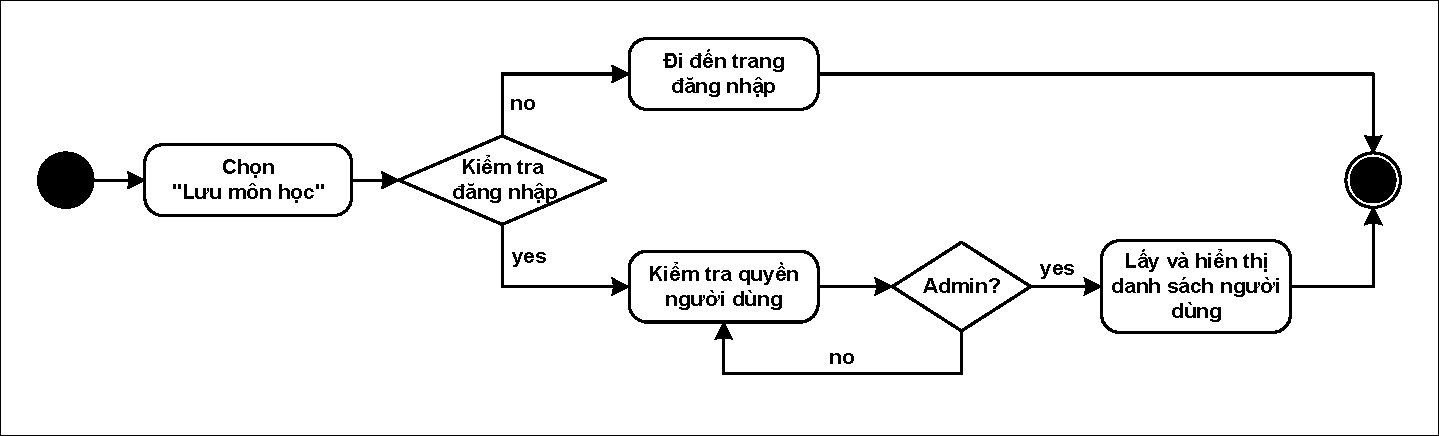
\includegraphics[trim= 10pt 10pt 10pt 10pt, clip, width=16cm]{activity_fig313.pdf}
		\caption [Biểu đồ Activity Diagram luồng hiển thị danh sách người dùng]{\bfseries \fontsize{12pt}{0pt}\selectfont Biểu đồ Activity Diagram luồng hiển thị danh sách người dùng}
		\label{fig313}
	\end{figure}
	
	\subsubsection{Chức năng xóa người dùng}
	
	Biểu đồ hoạt động luồng xử lý chức năng xóa người dùng trong hệ thống được biểu diễn trên Hình \ref{fig314}. Quá trình bắt đầu khi người quản trị chọn chức năng "Quản lý người dùng" trên giao diện quản trị. Hệ thống tiến hành kiểm tra trạng thái đăng nhập: nếu người dùng chưa đăng nhập, hệ thống sẽ điều hướng đến trang đăng nhập. Sau khi xác thực thành công, hệ thống tiếp tục kiểm tra quyền của người dùng. Chỉ những tài khoản có quyền quản trị (Admin) mới có thể tiếp tục thực hiện chức năng này.
	
	\begin{figure}[!ht]
		\centering
		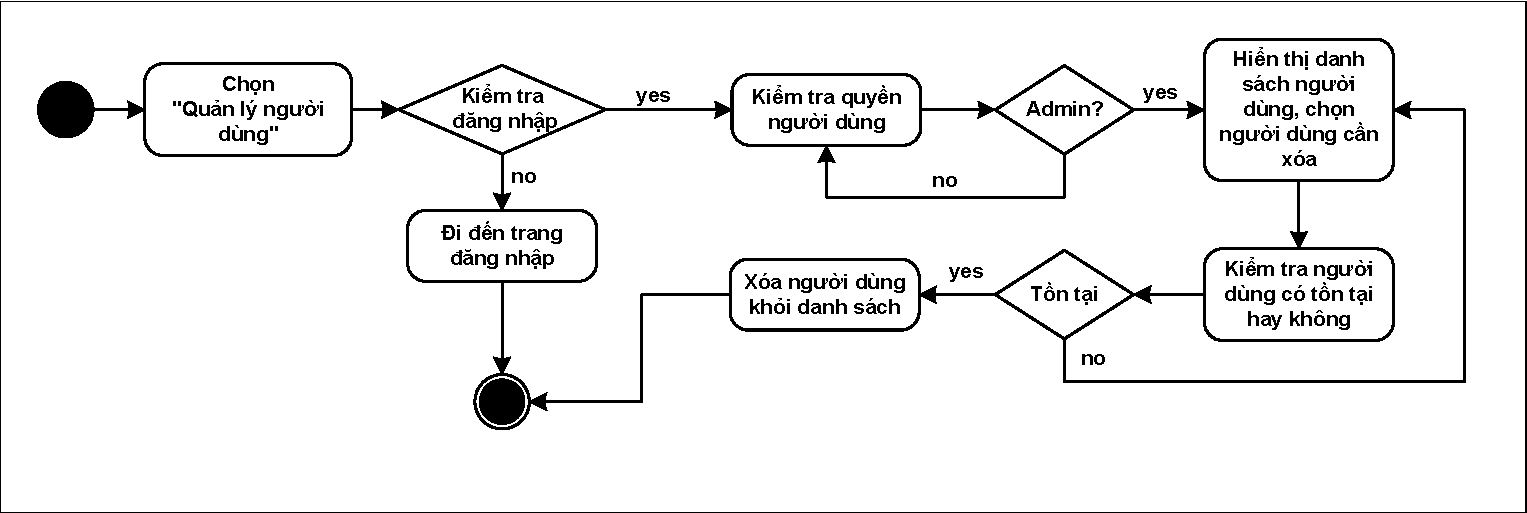
\includegraphics[trim= 10pt 10pt 10pt 10pt, clip, width=16cm]{activity_fig314.pdf}
		\caption [Biểu đồ Activity Diagram luồng xóa người dùng]{\bfseries \fontsize{12pt}{0pt}\selectfont Biểu đồ Activity Diagram luồng xóa người dùng}
		\label{fig314}
	\end{figure}
	
	Nếu quyền hợp lệ, hệ thống sẽ hiển thị danh sách người dùng hiện tại, cho phép quản trị viên lựa chọn đối tượng cần xóa. Sau đó, hệ thống tiến hành kiểm tra sự tồn tại của tài khoản được chọn. Nếu người dùng tồn tại, hệ thống sẽ thực hiện thao tác xóa khỏi cơ sở dữ liệu. Nếu không tồn tại, quá trình bị hủy bỏ và kết thúc. Việc kiểm tra quyền và sự tồn tại trước khi xóa nhằm đảm bảo tính an toàn và toàn vẹn dữ liệu hệ thống.
	
	\subsection{Biểu đồ tuần tự (Sequence Diagram)}
	
	Sequence diagram (biểu đồ tuần tự) là biểu đồ xác định trình tự diễn ra các sự kiện của một đối tượng hay một nhóm đối tượng. Nó miêu tả chi tiết thông tin gửi và nhận giữa các đối tượng, đồng thời chú trọng đến trình tự thời gian gửi và nhận của các thông tin đó.
	
	\subsubsection{Biểu đồ tuần tự chức năng đăng nhập}
	
	Biểu đồ tuần tự cho chức năng đăng nhập được biểu diễn trên Hình \ref{fig315}. Đầu tiên, người dùng nhập thông tin đăng nhập (tên đăng nhập và mật khẩu) thông qua giao diện View. Giao diện này gửi yêu cầu chứa thông tin đăng nhập đến Controller. Tại đây, Controller tiếp nhận và chuyển yêu cầu kiểm tra tính hợp lệ của thông tin đến Model (thường là service hoặc database access layer).
	
	Model kiểm tra dữ liệu người dùng và trả về kết quả xác thực:
	
	- Nếu thông tin hợp lệ, Controller điều hướng người dùng đến trang chủ, View sẽ hiển thị giao diện chính sau khi đăng nhập thành công.
	
	- Nếu thông tin không hợp lệ, Controller trả về thông báo lỗi, và View sẽ hiển thị thông báo này cho người dùng, yêu cầu nhập lại.
	
	\begin{figure}[!ht]
		\centering
		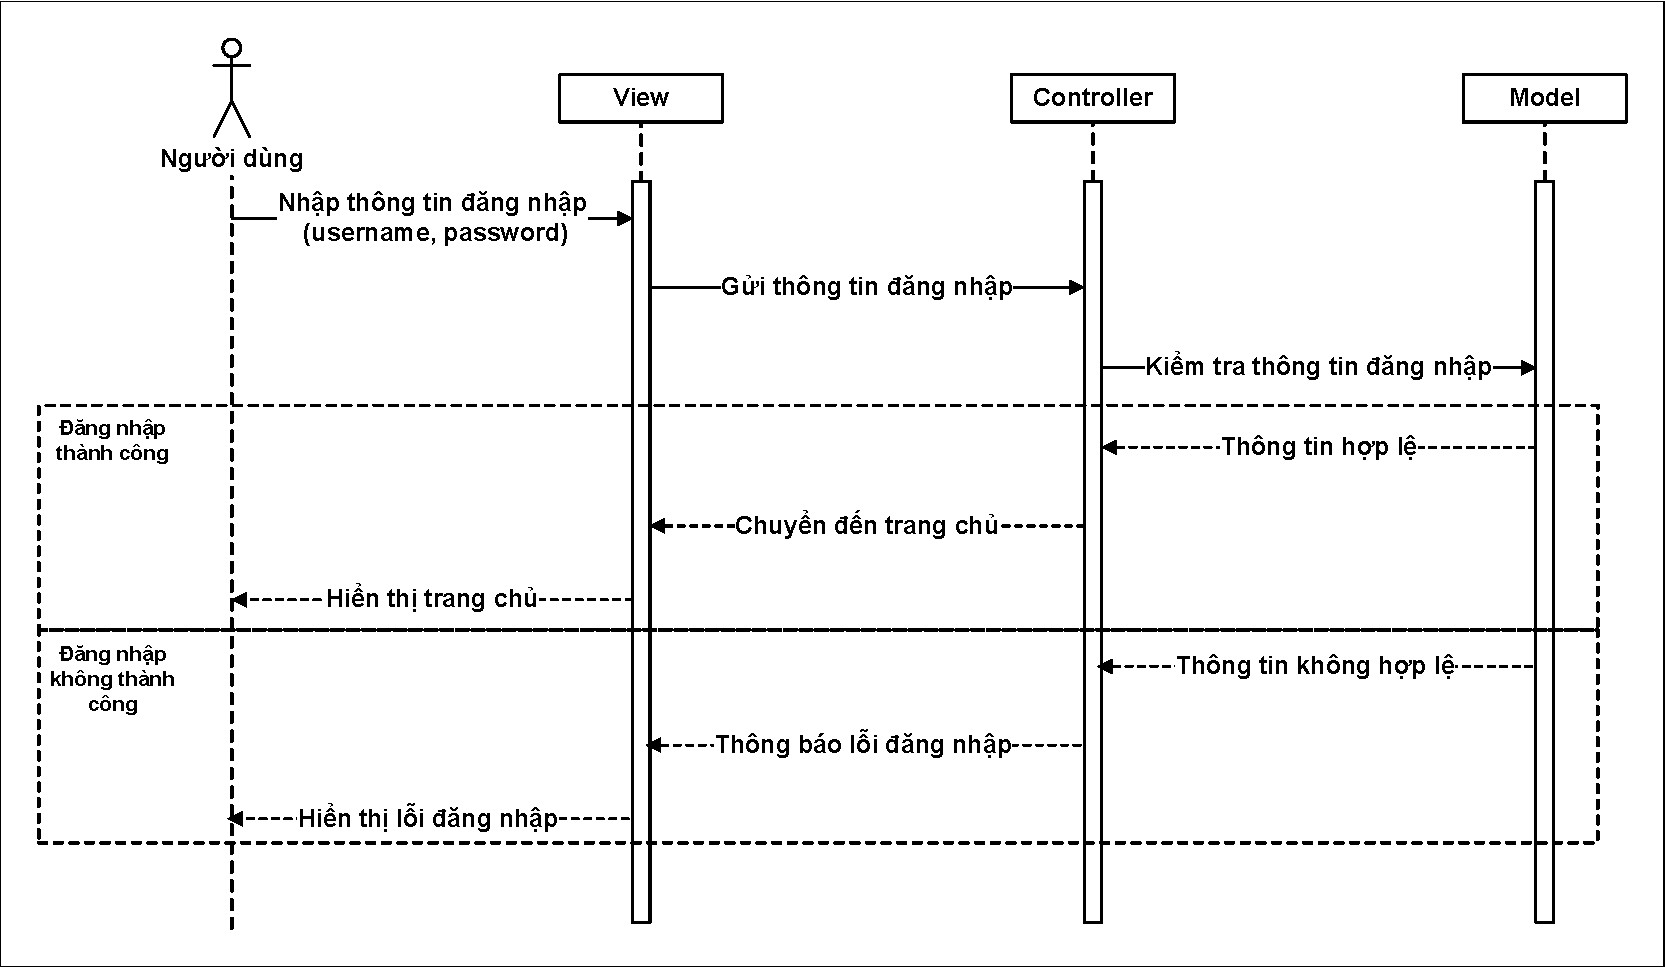
\includegraphics[trim= 10pt 10pt 10pt 10pt, clip, width=16cm]{sequence_fig315.pdf}
		\caption [Biểu đồ tuần tự chức năng đăng nhập]{\bfseries \fontsize{12pt}{0pt}\selectfont Biểu đồ tuần tự chức năng đăng nhập}
		\label{fig315}
	\end{figure}
	
	\subsubsection{Biểu đồ tuần tự chức năng đăng ký}
	
	\begin{figure}[!ht]
		\centering
		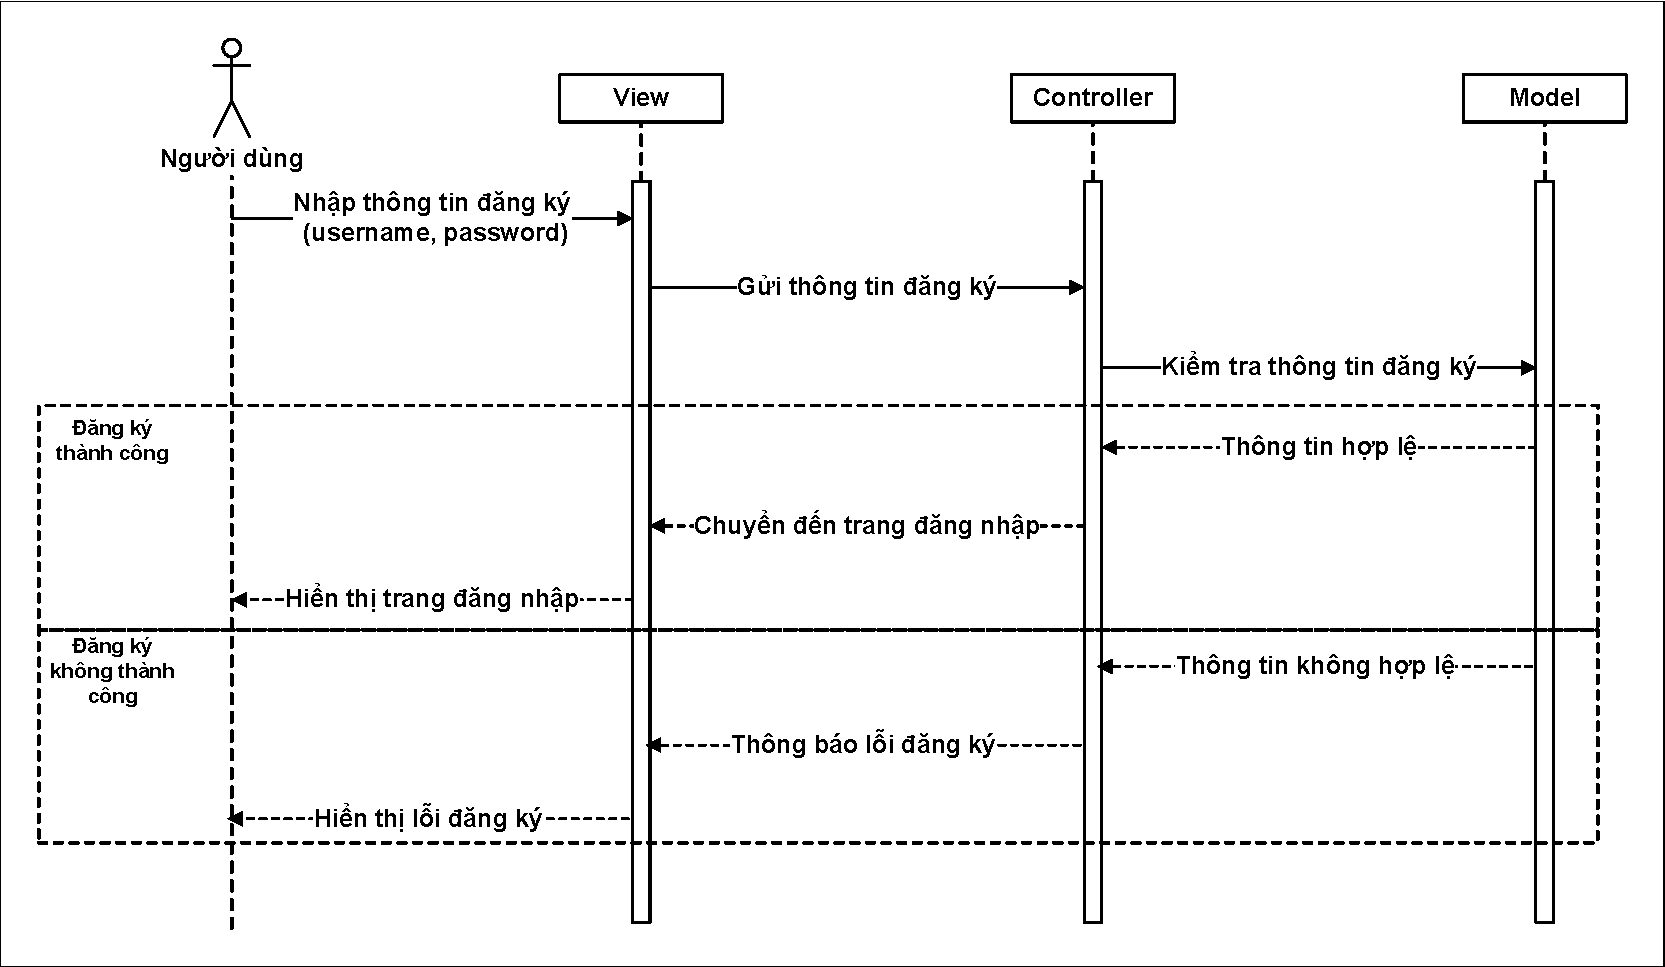
\includegraphics[trim= 10pt 10pt 10pt 10pt, clip, width=16cm]{sequence_fig316_1.pdf}
		\caption [Biểu đồ tuần tự chức năng đăng ký]{\bfseries \fontsize{12pt}{0pt}\selectfont Biểu đồ tuần tự chức năng đăng ký}
		\label{fig316}
	\end{figure}
	
	Biểu đồ tuần tự cho chức năng đăng ký được biểu diễn trên Hình \ref{fig316}. Người dùng bắt đầu bằng cách nhập thông tin đăng ký cơ bản (họ tên, tên đăng nhập, mật khẩu...) vào giao diện (View). Sau đó, View gửi toàn bộ dữ liệu đăng ký đến Controller để xử lý. Tại Controller, dữ liệu này được xác minh sơ bộ (như kiểm tra định dạng, độ dài mật khẩu...) và được chuyển tiếp sang Model để thực hiện các kiểm tra sâu hơn như: tài khoản đã tồn tại hay chưa, username có trùng không, v.v.
	
	Tùy thuộc vào kết quả từ Model:
	
	- Nếu thông tin đăng ký hợp lệ và chưa từng tồn tại, hệ thống sẽ tiến hành lưu thông tin người dùng mới vào cơ sở dữ liệu, và Controller sẽ chuyển hướng người dùng đến trang đăng nhập kèm theo thông báo đăng ký thành công.
	
	- Ngược lại, nếu có lỗi (ví dụ: tài khoản đã tồn tại), Controller sẽ trả về thông báo lỗi, và View sẽ hiển thị để người dùng biết và nhập lại.
	
	\subsubsection{Biểu đồ tuần tự chức năng đăng ký môn học}
	
	Biểu đồ tuần tự cho chức năng đăng ký môn học được biểu diễn trên Hình \ref{fig317}. 
	
	\begin{figure}[!ht]
		\centering
		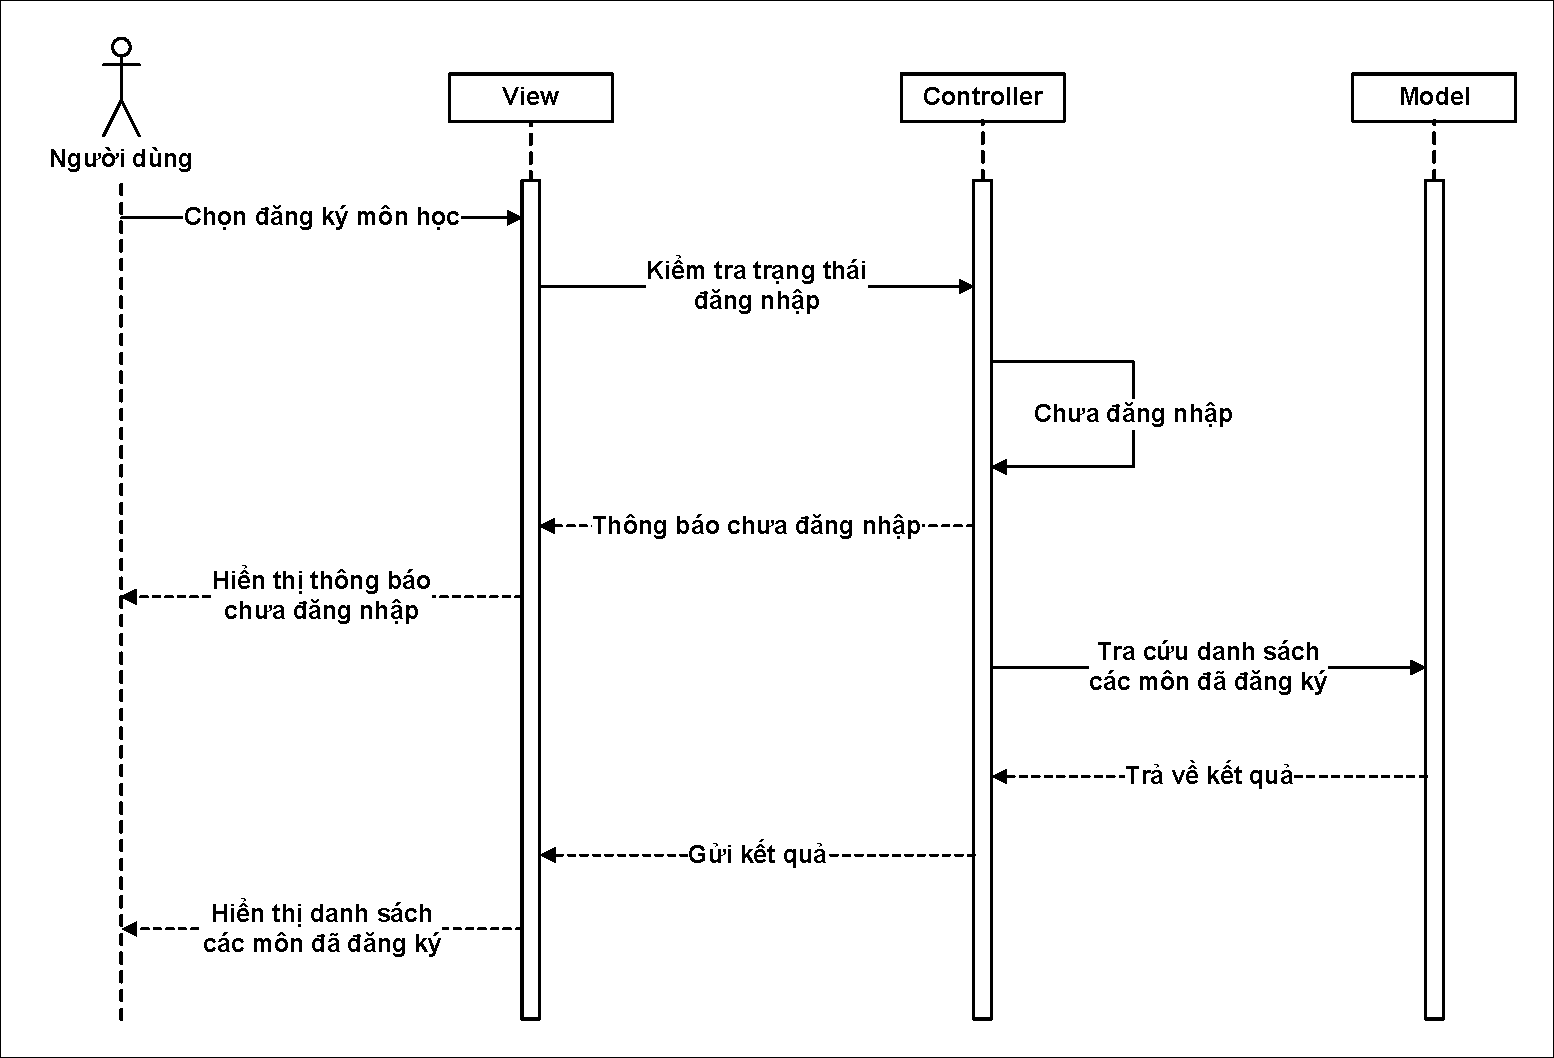
\includegraphics[trim= 10pt 10pt 10pt 10pt, clip, width=16cm]{sequence_fig317.pdf}
		\caption [Biểu đồ tuần tự chức năng đăng ký môn học]{\bfseries \fontsize{12pt}{0pt}\selectfont Biểu đồ tuần tự chức năng đăng ký môn học}
		\label{fig317}
	\end{figure}
	
	 Khi người dùng chọn chức năng đăng ký môn học, hệ thống sẽ kiểm tra trạng thái đăng nhập. Nếu người dùng chưa đăng nhập, giao diện sẽ hiển thị thông báo yêu cầu đăng nhập. Ngược lại, nếu đã đăng nhập, Controller sẽ gửi yêu cầu đến Model để tra cứu danh sách các môn học mà người dùng đã đăng ký. Kết quả sau đó được trả về giao diện và hiển thị cho người dùng. Biểu đồ này phản ánh quá trình xử lý hợp lý và đảm bảo kiểm tra quyền truy cập trước khi truy xuất dữ liệu học phần.
	 
	 \subsubsection{Biểu đồ tuần tự chức năng lưu môn học}
	 
	 Biểu đồ tuần tự cho chức năng lưu môn học được biểu diễn trên Hình \ref{fig318}. Khi người dùng chọn thao tác lưu môn học, View sẽ gửi yêu cầu đến Controller để xử lý. Controller tiến hành kiểm tra trạng thái đăng nhập của người dùng. Nếu người dùng chưa đăng nhập, hệ thống sẽ phản hồi bằng thông báo yêu cầu đăng nhập. Nếu đã đăng nhập, Controller sẽ gửi yêu cầu lưu môn học đến Model. Sau khi Model xử lý và xác nhận lưu thành công, kết quả sẽ được phản hồi về Controller rồi chuyển đến View để thông báo cho người dùng. Biểu đồ thể hiện rõ tính bảo mật và trình tự hợp lý trong thao tác lưu trữ dữ liệu người dùng.
	 
	 \begin{figure}[!ht]
	 	\centering
	 	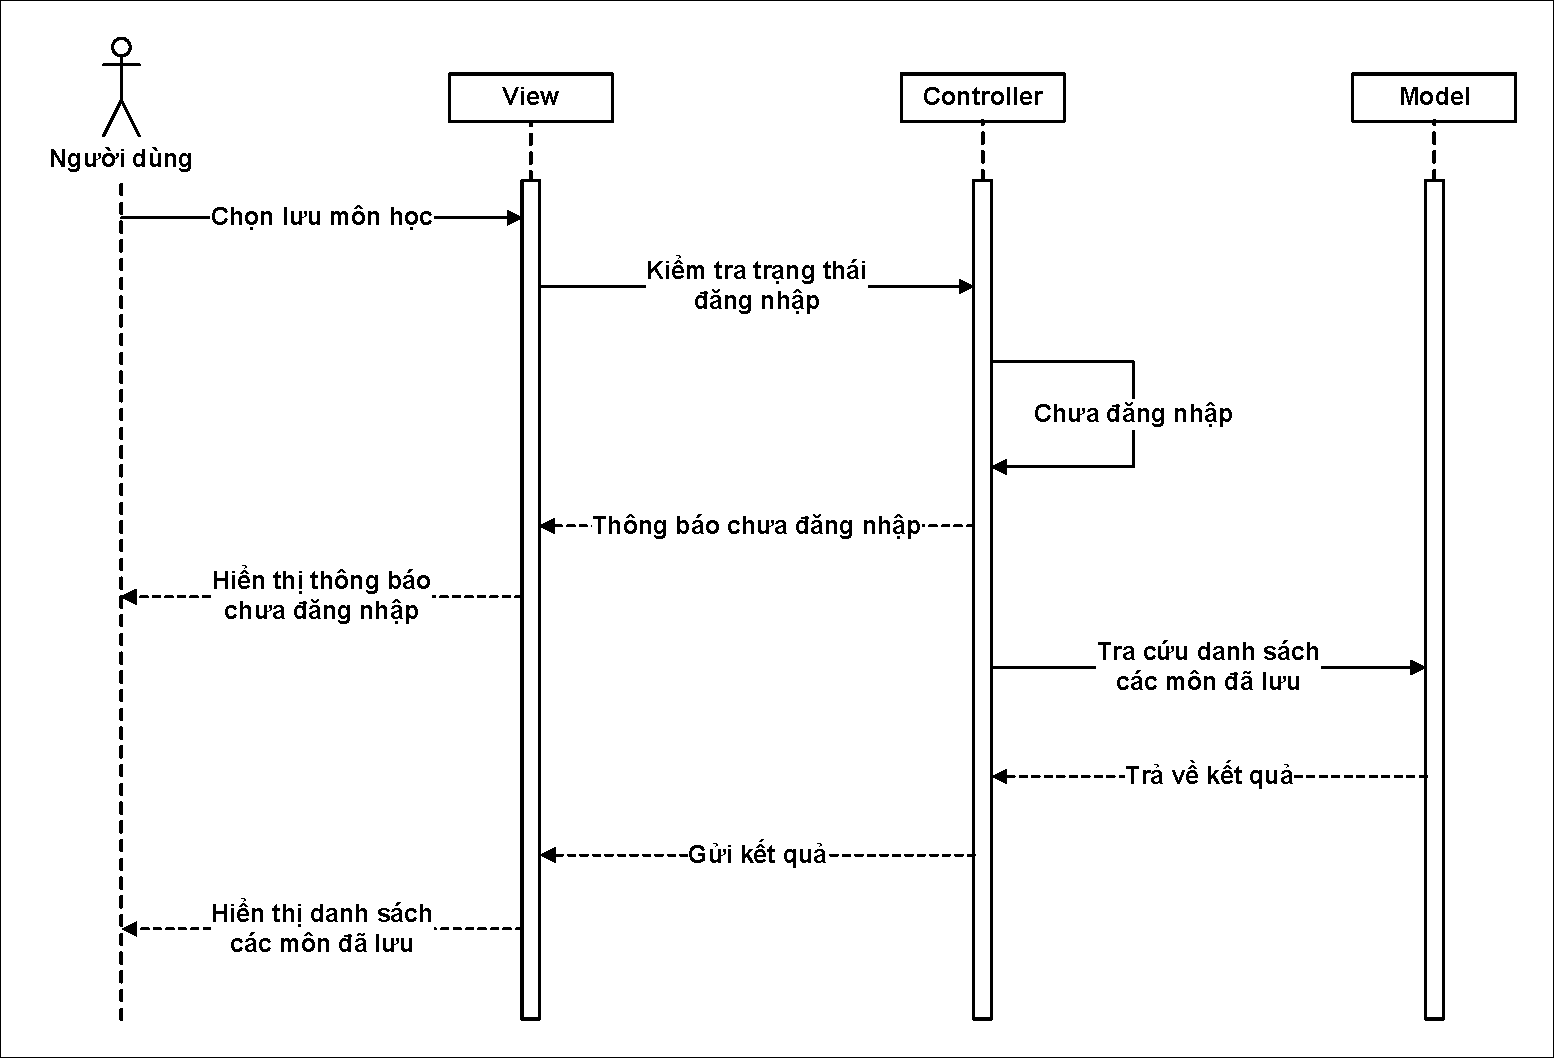
\includegraphics[trim= 10pt 10pt 10pt 10pt, clip, width=16cm]{sequence_fig318_1.pdf}
	 	\caption [Biểu đồ tuần tự chức năng lưu môn học]{\bfseries \fontsize{12pt}{0pt}\selectfont Biểu đồ tuần tự chức năng lưu môn học}
	 	\label{fig318}
	 \end{figure}
	 
	 \subsubsection{Biểu đồ tuần tự chức năng hiển thị danh sách người dùng}
	 
	 Biểu đồ tuần tự cho chức năng hiển thị danh sách người dùng được biểu diễn trên Hình \ref{fig319}. Khi người dùng chọn thao tác hiển thị danh sách người dùng, View sẽ gửi yêu cầu đến Controller để xử lý. Controller tiến hành kiểm tra trạng thái đăng nhập của người dùng. Nếu người dùng chưa đăng nhập, Controller sẽ thông báo cho View, và View sẽ hiển thị thông báo yêu cầu đăng nhập đến người dùng.
	 
	 Nếu người dùng đã đăng nhập, Controller tiếp tục kiểm tra quyền hạn của người dùng. Trong trường hợp người dùng không phải là quản trị viên, Controller sẽ gửi kết quả về View, và View sẽ thông báo rằng không thể hiển thị danh sách người dùng. Chỉ khi người dùng đã đăng nhập và có quyền quản trị viên, Controller mới gửi yêu cầu đến Model để lấy danh sách người dùng. Sau khi Model xử lý và trả về danh sách, kết quả sẽ được phản hồi về Controller rồi chuyển đến View để hiển thị cho người dùng.
	 
	 \begin{figure}[!ht]
	 	\centering
	 	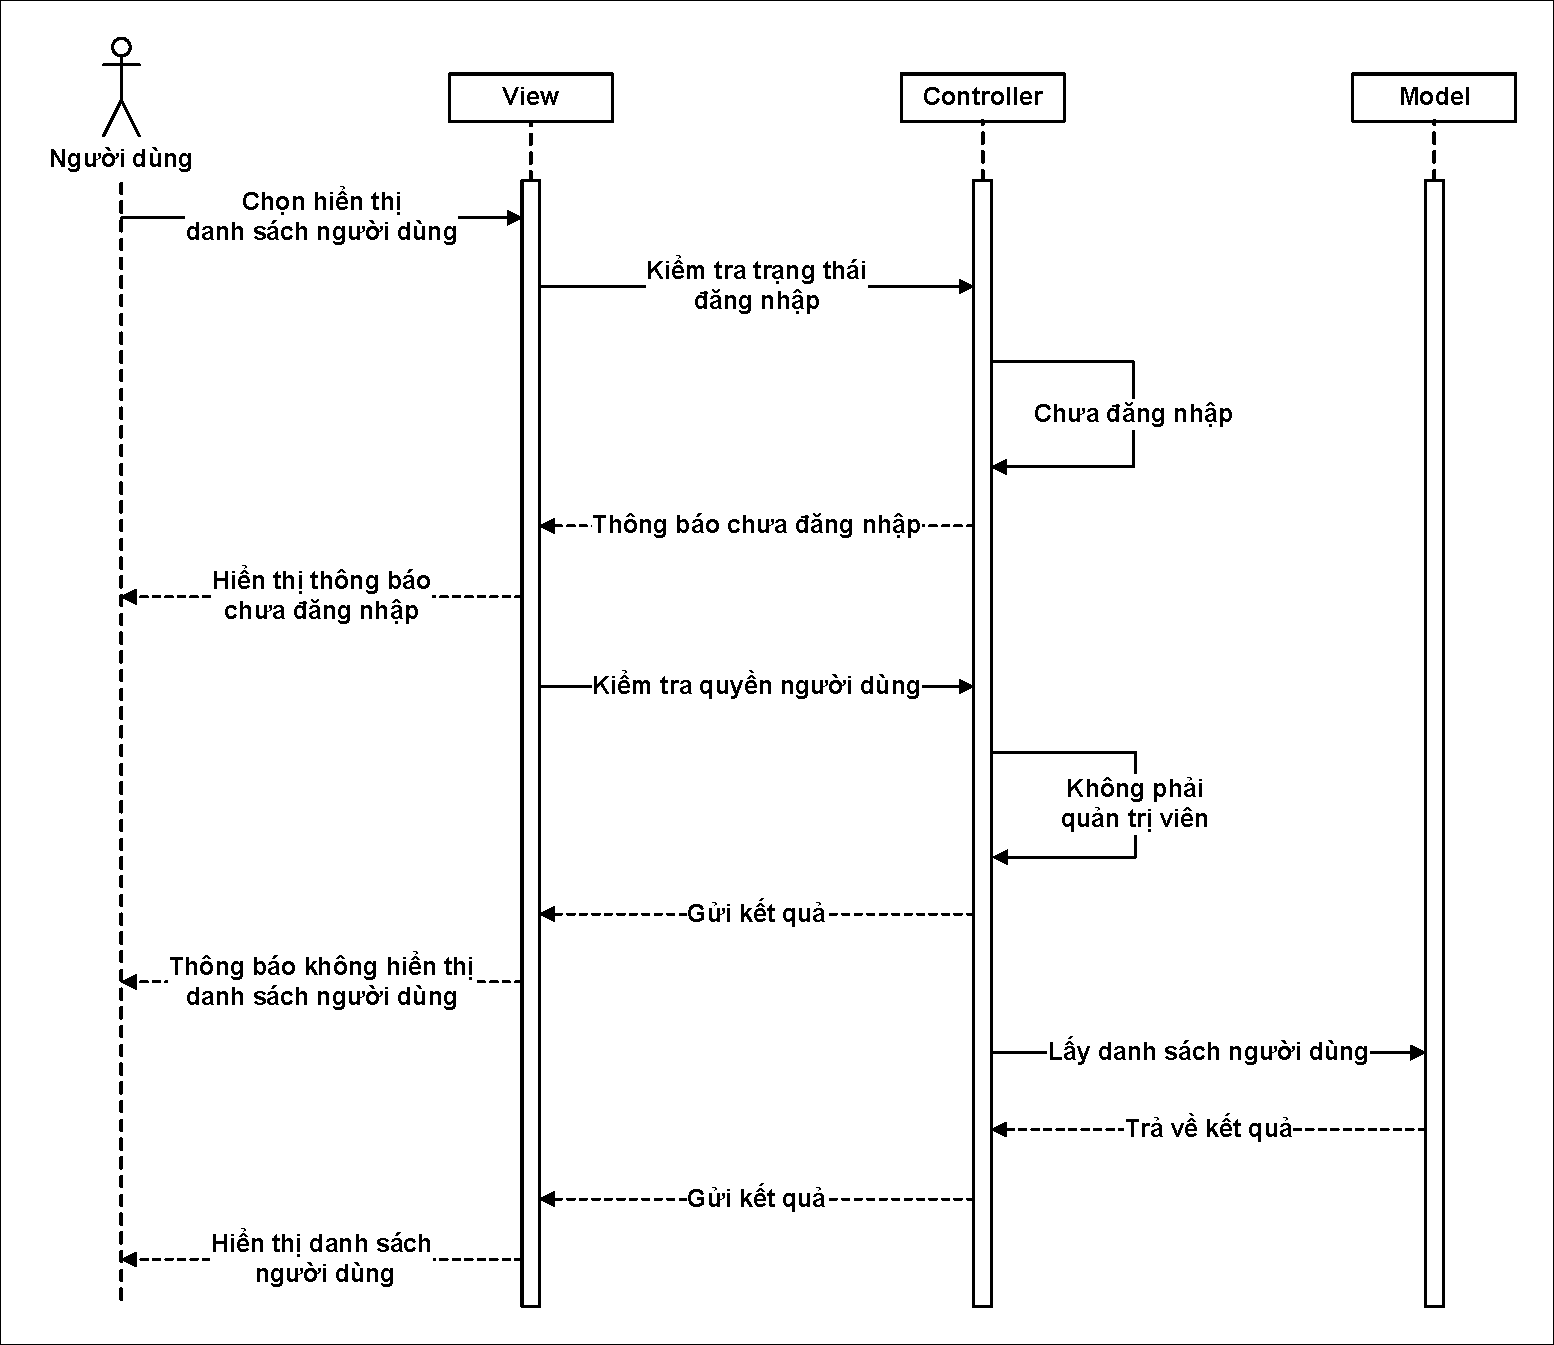
\includegraphics[trim= 10pt 10pt 10pt 10pt, clip, width=16cm]{sequence_fig319_1.pdf}
	 	\caption [Biểu đồ tuần tự chức năng hiển thị danh sách người dùng]{\bfseries \fontsize{12pt}{0pt}\selectfont Biểu đồ tuần tự chức năng hiển thị danh sách người dùng}
	 	\label{fig319}
	 \end{figure}
	 
	 \subsubsection{Biểu đồ tuần tự chức năng xóa người dùng}
	 
	 Biểu đồ tuần tự cho chức năng xóa người dùng được biểu diễn trên Hình \ref{fig320}. Khi người dùng chọn thao tác xóa người dùng, View sẽ gửi yêu cầu đến Controller để xử lý. Controller tiến hành kiểm tra trạng thái đăng nhập của người dùng. Nếu người dùng chưa đăng nhập, Controller sẽ thông báo cho View, và View sẽ hiển thị thông báo yêu cầu đăng nhập đến người dùng.
	 
	 \begin{figure}[!ht]
	 	\centering
	 	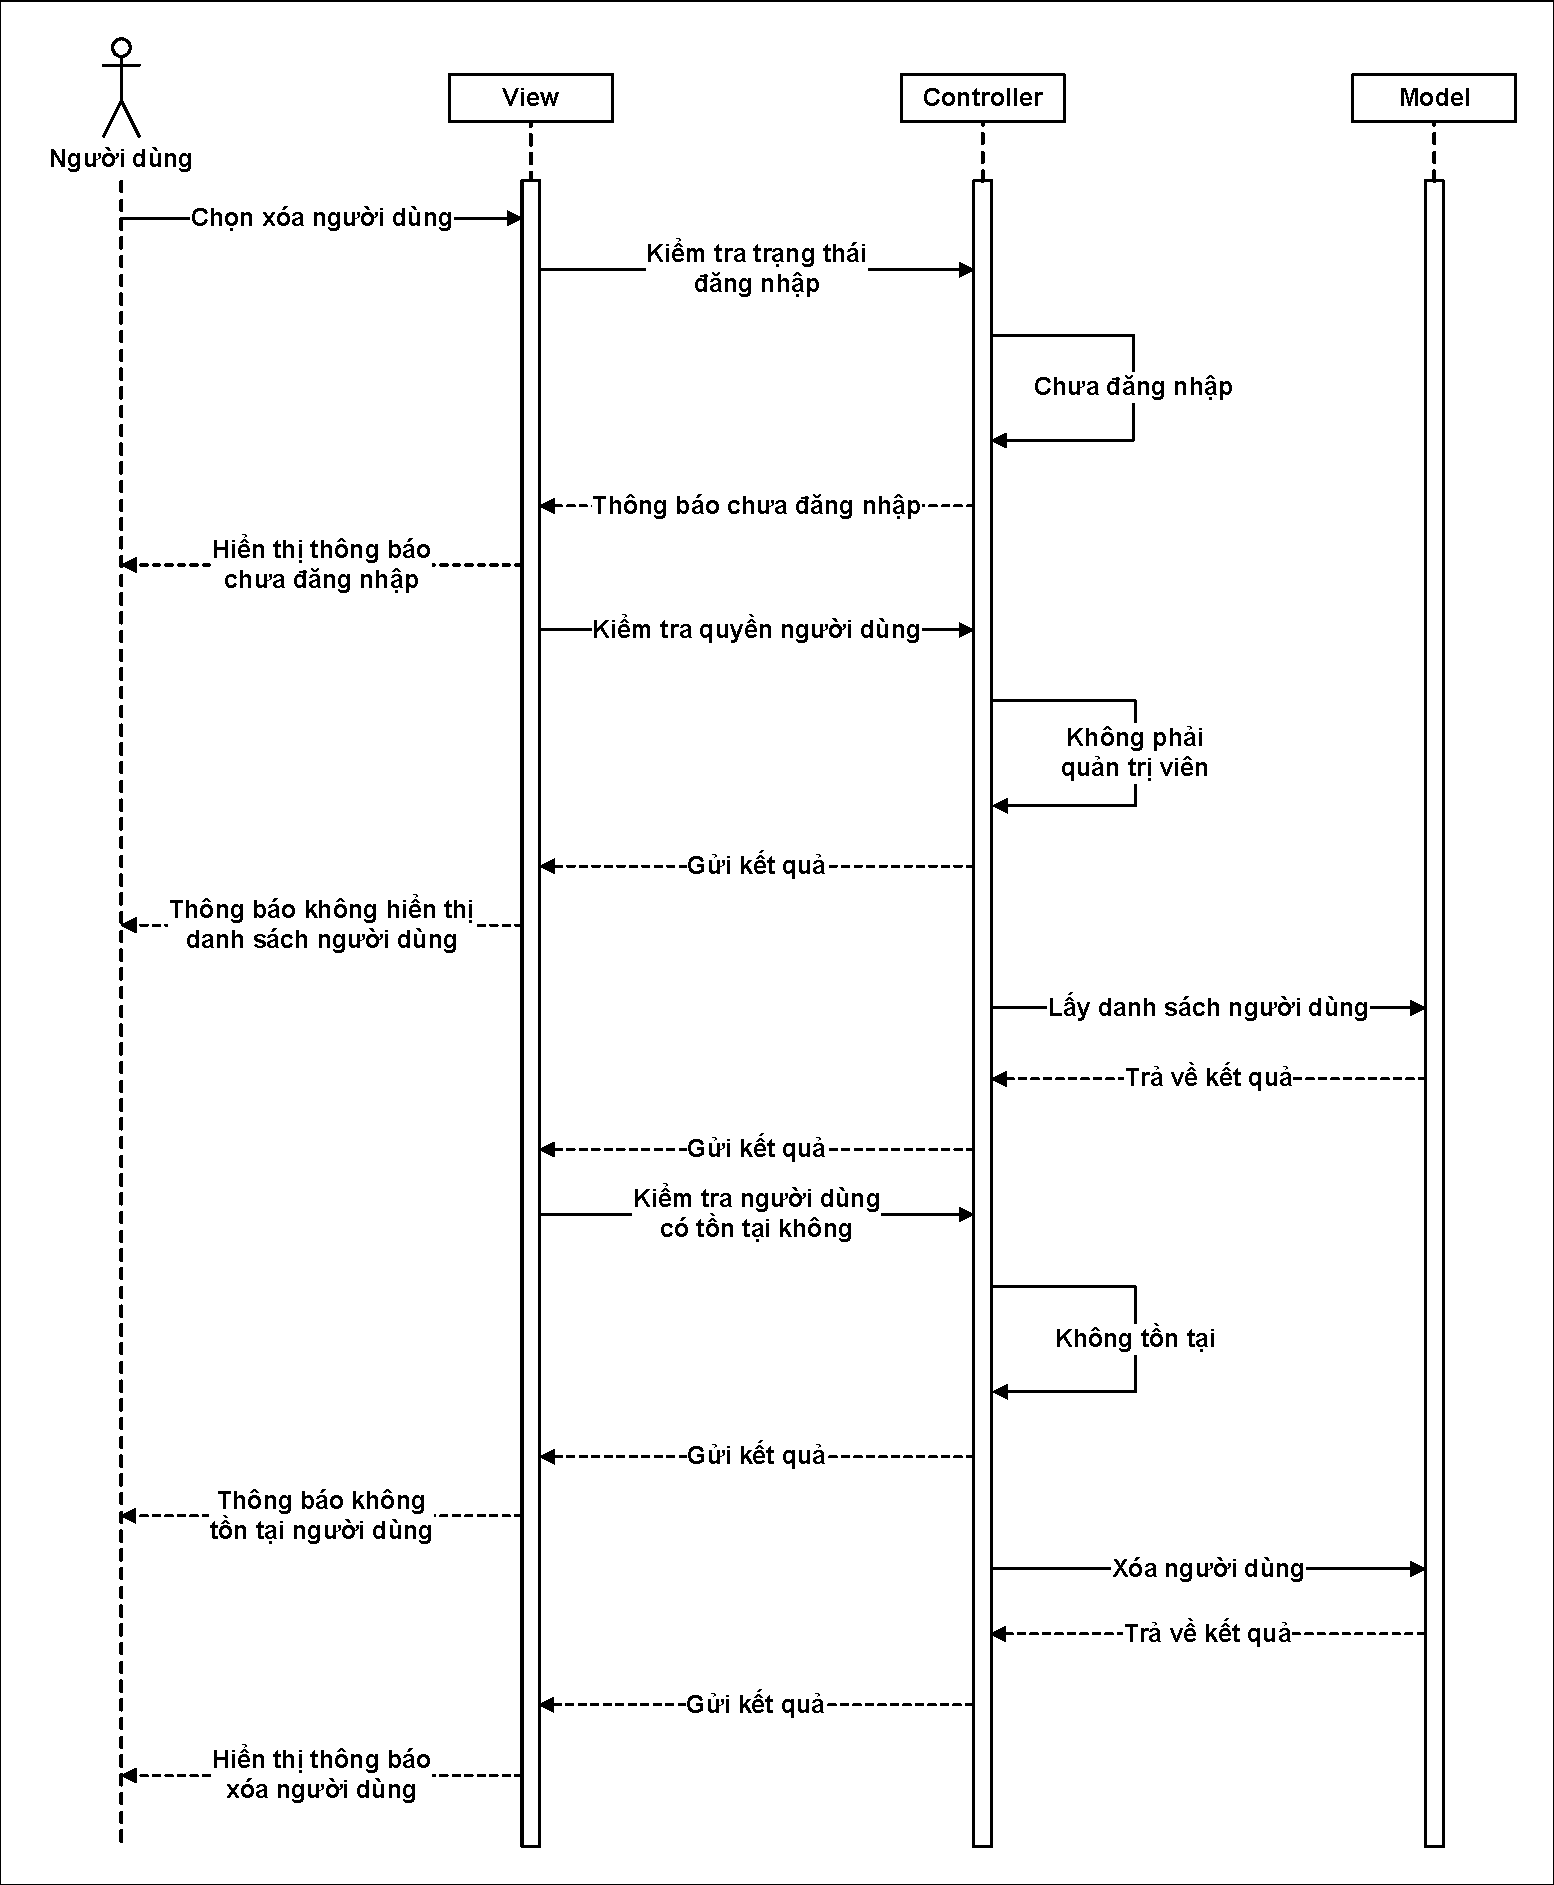
\includegraphics[trim= 10pt 10pt 10pt 10pt, clip, width=16cm]{sequence_fig320.pdf}
	 	\caption [Biểu đồ tuần tự chức năng xóa người dùng]{\bfseries \fontsize{12pt}{0pt}\selectfont Biểu đồ tuần tự chức năng xóa người dùng}
	 	\label{fig320}
	 \end{figure}
	 
	 Nếu người dùng đã đăng nhập, Controller tiếp tục kiểm tra quyền hạn của người dùng. Trong trường hợp người dùng không phải là quản trị viên, Controller sẽ gửi kết quả về View, và View sẽ thông báo rằng không thể hiển thị danh sách người dùng (theo như văn bản trên biểu đồ). Chỉ khi người dùng đã đăng nhập và có quyền quản trị viên, Controller sẽ tiếp tục các bước xử lý. Đầu tiên, Controller có thể lấy danh sách người dùng từ Model (hoặc đây là bước chuẩn bị để xác định người dùng cần xóa). Sau đó, Controller sẽ kiểm tra xem người dùng cần xóa có tồn tại hay không. Nếu người dùng không tồn tại, Controller sẽ gửi kết quả về View, và View sẽ hiển thị thông báo rằng không tồn tại người dùng.
	 
	 Trong trường hợp người dùng tồn tại, Controller sẽ gửi yêu cầu xóa người dùng đến Model. Sau khi Model xử lý và xác nhận xóa thành công, kết quả sẽ được phản hồi về Controller rồi chuyển đến View để hiển thị thông báo xóa người dùng đến người dùng.
	 
	 \subsection{Sơ đồ thực thể liên kết (ERD)}
	 \subsubsection{Các thực thể, thuộc tính}
	 
	 \begin{table}[H]
	 	\centering
	 	\caption [Bảng thực thể và thuộc tính của hệ thống]{\bfseries \fontsize{12pt}{0pt}\selectfont Bảng thực thể và thuộc tính của hệ thống}
	 	\label{tab311}
	 	\begin{tabular}{|p{6cm}|p{8.5cm}|}
	 		\hline
	 		\textbf{Thực thể} & \textbf{Thuộc tính} \\
	 		\hline
	 		users & username, password, fullname, dob, gender, role, status, avatar \\
	 		\hline
	 		courses & course\_id, course\_name, english\_name, child\_management, managing\_department, weight, description, price, thumbnail, author \\
	 		\hline
	 		documents & doc\_id, course, title, file\_url, upload\_date, type\_doc, doc\_author \\
	 		\hline
	 		user\_courses & id, username, course\_id, registered\_at \\
	 		\hline
	 		user\_like\_courses & id, username, course\_id, liked\_at \\
	 		\hline
	 	\end{tabular}
	 \end{table}
	 
	 \subsubsection{Mô hình quan hệ}
	 \begin{figure}[!ht]
	 	\centering
	 	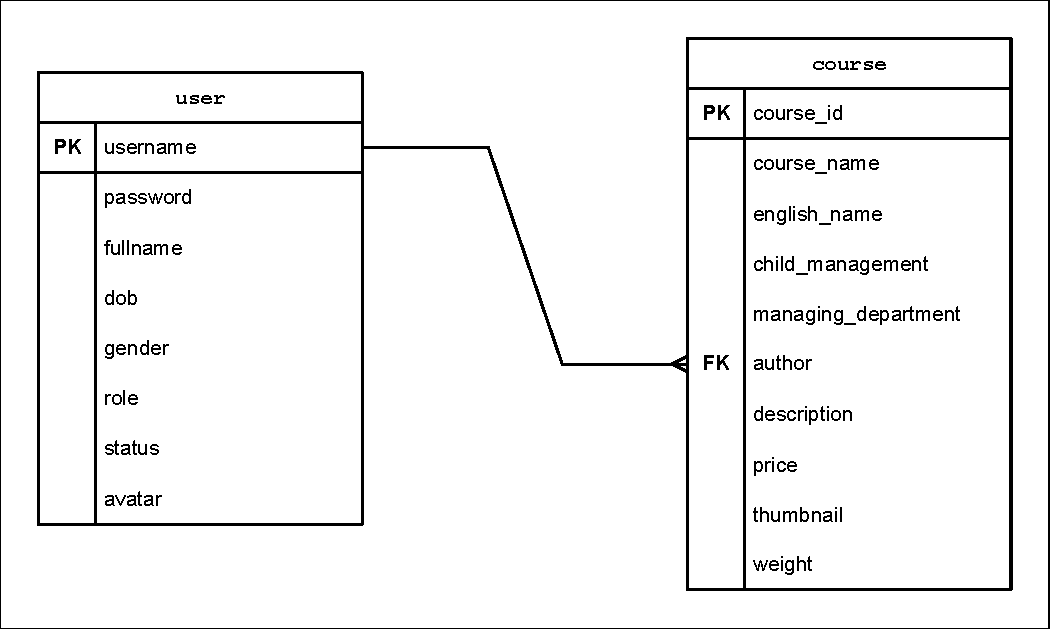
\includegraphics[trim= 10pt 10pt 10pt 10pt, clip, width=14cm]{edr_fig321_1.pdf}
	 	\caption [Quan hệ giữa người dùng và môn học]{\bfseries \fontsize{12pt}{0pt}\selectfont Quan hệ giữa người dùng và môn học}
	 	\label{fig321}
	 \end{figure}
	 
	 Hình \ref{fig321} thể hiện mối quan hệ giữa các thực thể: người dùng và môn học. Cụ thể: Một người dùng có thể là tác giả của nhiều khóa học. Một khóa học chỉ được tạo ra bởi một người dùng.
	 
	 \begin{figure}[!ht]
	 	\centering
	 	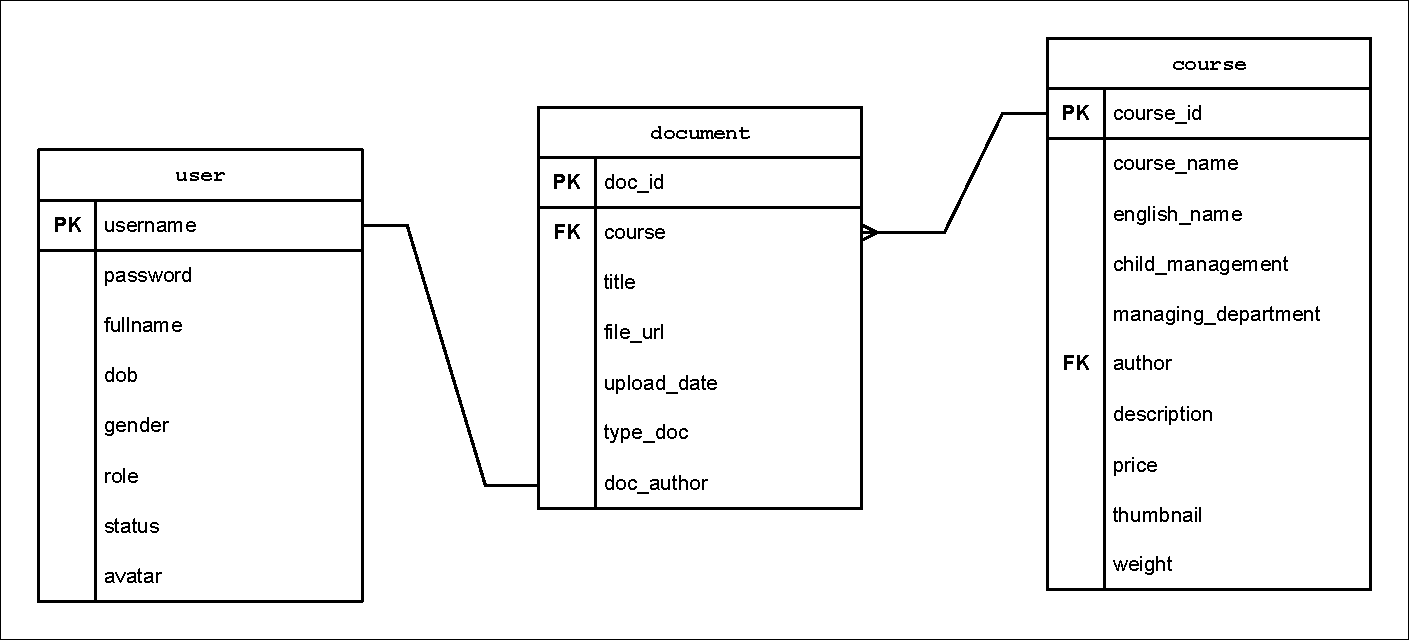
\includegraphics[trim= 10pt 10pt 10pt 10pt, clip, width=15.5cm]{edr_fig322_1.pdf}
	 	\caption [Quan hệ giữa người dùng, môn học và tài liệu]{\bfseries \fontsize{12pt}{0pt}\selectfont Quan hệ giữa người dùng, môn học và tài liệu}
	 	\label{fig322}
	 \end{figure}
	 
	 Hình \ref{fig322} thể hiện mối quan hệ giữa các thực thể: người dùng, môn học và tài liệu. Cụ thể: Một người dùng là tác giả của một tài liệu, và một tài liệu chỉ có một người là tác giả. Một khóa học có thể có nhiều tài liệu, nhưng một tài liệu nhất định chỉ thuộc về một môn học.
	 
	 \begin{figure}[!ht]
	 	\centering
	 	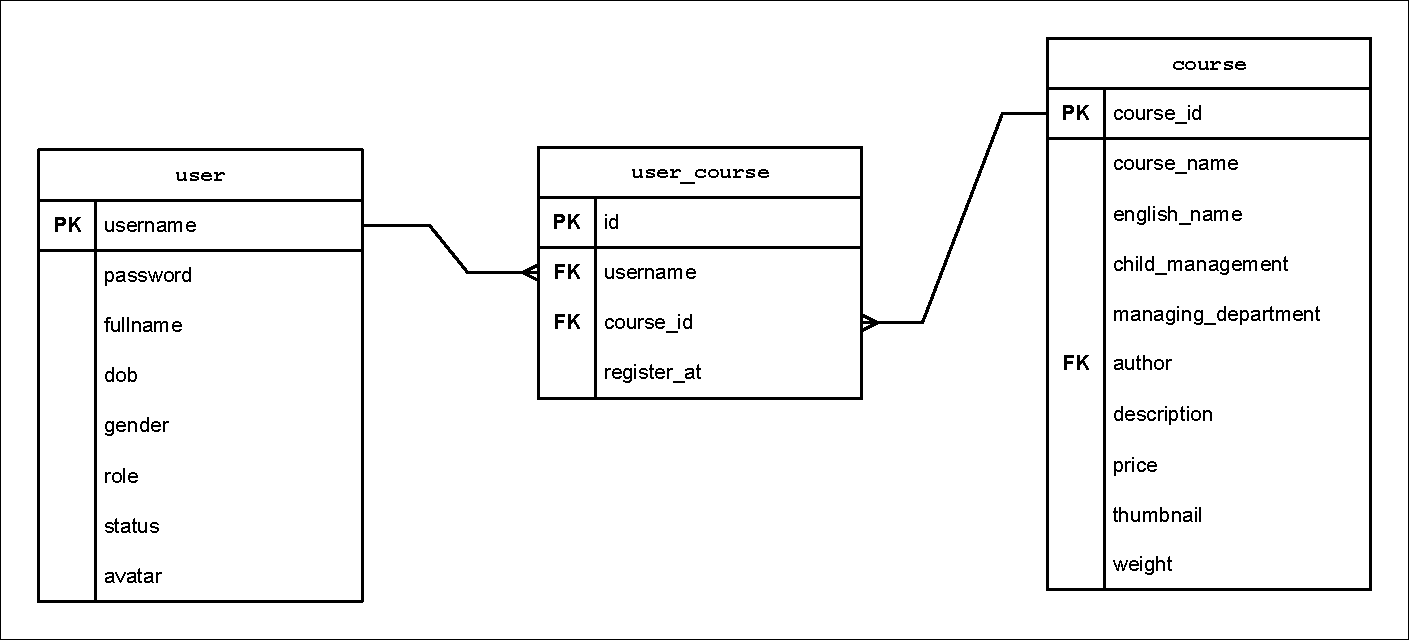
\includegraphics[trim= 10pt 10pt 10pt 10pt, clip, width=15.5cm]{edr_fig323.pdf}
	 	\caption [Quan hệ giữa người dùng, môn học và danh sách môn học đã đăng ký]{\bfseries \fontsize{12pt}{0pt}\selectfont Quan hệ giữa người dùng, môn học và danh sách môn học đã đăng ký}
	 	\label{fig323}
	 \end{figure}
	 
	 Hình \ref{fig323} thể hiện mối quan hệ giữa các thực thể: người dùng, môn học và danh sách môn học đã đăng ký. Cụ thể: Một người dùng có thể đăng ký nhiều khóa học, và một khóa học có thể đăng ký bởi nhiều người.
	 
	 \begin{figure}[!ht]
	 	\centering
	 	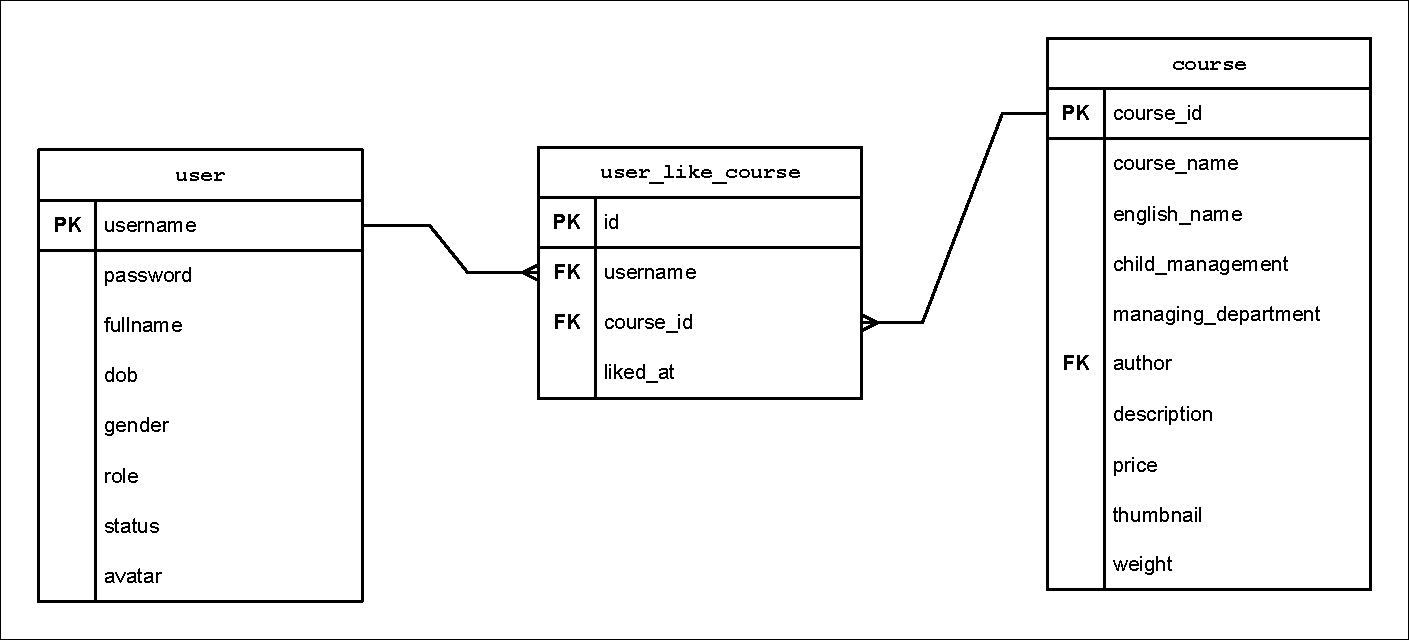
\includegraphics[trim= 10pt 10pt 10pt 10pt, clip, width=15.5cm]{edr_fig324.pdf}
	 	\caption [Quan hệ giữa người dùng, môn học và danh sách môn học đã lưu]{\bfseries \fontsize{12pt}{0pt}\selectfont Quan hệ giữa người dùng, môn học và danh sách môn học đã lưu}
	 	\label{fig324}
	 \end{figure}
	 
	 Hình \ref{fig324} thể hiện mối quan hệ giữa các thực thể: người dùng, môn học và danh sách môn học đã lưu. Cụ thể: Một người dùng có thể lưu nhiều khóa học, và một khóa học có thể lưu bởi nhiều người.
	 
	 \subsection{Xây dựng sơ đồ lớp (Class Diagram)}
	 
	 Class diagram (sơ đồ lớp) là khối xây dựng chính trong thiết kế hệ thống hướng đối tượng. Sơ đồ biểu diễn các lớp trong hệ thống, các thuộc tính và tính năng của mỗi lớp và mối quan hệ giữa các lớp. Hầu hết khi thiết kế hệ thống, một lớp có ba phần: tên lớp, các thuộc tính của lớp, các tính năng của lớp đó.
\end{document}